\chapter{Reproducible and open library}
\label{chap:peerannot}
\enlargethispage{3\baselineskip}

\begin{keypointstwomargins}{Reproducible and open library}{-2cm}{-1cm}
        \textbf{Key points -- Community based data but what about codes\dots}
        \begin{enumerate}[leftmargin=*]
        \item Reproducibility has been a demand from the scientific community. With crowdsourcing, the coupling of the label-gathering step and the aggregation is key to creating a classical supervised learning dataset. Different label aggregation strategies can lead to widely different results. Releasing publicly available datasets' original version with collected labels would lead to better data quality and better understanding of aggregation strategies.
        \item More than the data itself, as the crowdsourcing community is made of researchers with very diverse backgrounds, new models arise quickly. In multiple coding languages (if any) and with personalized data formats. We need formatting propositions that can handle large datasets, are easily accessible and understandable.
        \item Aggregation strategies are often EM-based with a two-step procedure repeated. While performance is an important decision factor in using one strategy over another, how much time it takes to run is essential. Especially with large datasets, we find memory scaling issues or a time complexity that forbids usage in applications.
        \end{enumerate}

        \textbf{Contributions -- peerannot and Benchopt}
        \begin{enumerate}[leftmargin=*,start=4]
        \item We propose a new \texttt{python} library \texttt{peerannot} fully documented. An \texttt{identify} module lets users identify ambiguous tasks from datasets using a wide range of strategies. The \texttt{aggregate} module performs label aggregation strategies. The \texttt{aggregate-deep} module uses learning strategies that are deep-learning based and have inserted the aggregation step inside the network's architecture. The \texttt{train} module allows to train classifiers from aggregated labels. Our library comes with data templates and examples available at \url{http://peerannot.github.io}
        \item We created a crowdsourcing benchmark in the \texttt{BenchOpt} library to easily compare time performance on label aggregation strategies across libraries, on publicly available datasets.
        \end{enumerate}
\end{keypointstwomargins}

\section{\texttt{peerannot}: Open access for crowdsourcing strategies in python}

The experiments ran in \Cref{chap:waum} made us realize key points in the field of crowdsourcing. The first one is that the data is often not released in a format that is easily usable -- when released. The second is that most of the time, the code is not released -- or partially released without functions and easy access to run new experiments, or also scattered with each their different programming language (\texttt{python}, R, stan, java,\dots). The third is that existing libraries to handle crowdsourcing data lack implemented strategies to identify poorly performing workers and/or ambiguous tasks.
Thus, we created the \texttt{peerannot} library.

Crowdsourced datasets induce at least three major challenges to which we contribute with \texttt{peerannot}:

\begin{enumerate}
  \item \textbf{How to aggregate multiple labels into a single label from crowdsourced tasks?} This occurs, for example, when dealing with a single dataset that has been labeled by multiple workers with disagreements. This is also encountered with other scoring issues such as polls, reviews, peer-grading, \textit{etc.} In our framework, this is treated with the \texttt{aggregate} command, which given multiple labels, infers a label. From aggregated labels, a classifier can then be trained using the \texttt{train} command.
  \item \textbf{How to learn a classifier from crowdsourced datasets?} Where the first question is bound by aggregating multiple labels into a single one, this considers the case where we do not need a single label to train on, but instead train a classifier on the crowdsourced data, with the motivation to perform well on a testing set. This end-to-end vision is common in machine learning; however, it requires the actual tasks (the images, texts, videos, \textit{etc.}) to train on -- and in crowdsourced datasets publicly available, they are not always available. This is treated with the \texttt{aggregate-deep} command that runs strategies where the aggregation has been transformed into a deep learning optimization problem.
  \item \textbf{How to identify good workers in the crowd and difficult tasks?} When multiple answers are given to a single task, looking for who to trust for which type of task becomes necessary to estimate the labels or later train a model with as few noise sources as possible. The module \texttt{identify} uses different scoring metrics to create a worker and/or task evaluation.
\end{enumerate}

The library \texttt{peerannot} addresses these practical questions within a reproducible setting and an easy-to-follow pipeline presented in \Cref{fig:pipeline_crowdsourcing_peerannot}. Indeed, the complexity of experiments often leads to a lack of transparency and reproducible results for simulations and real datasets.
We propose standard simulation settings with explicit implementation parameters that can be shared.
For real datasets, \texttt{peerannot} is compatible with standard neural network architectures from the \texttt{Torchvision} \citep{torchvision} library and \texttt{Pytorch} \citep{pytorch}, allowing a flexible framework with easy-to-share scripts to reproduce experiments.

\begin{figure}[ht]
        \centering
        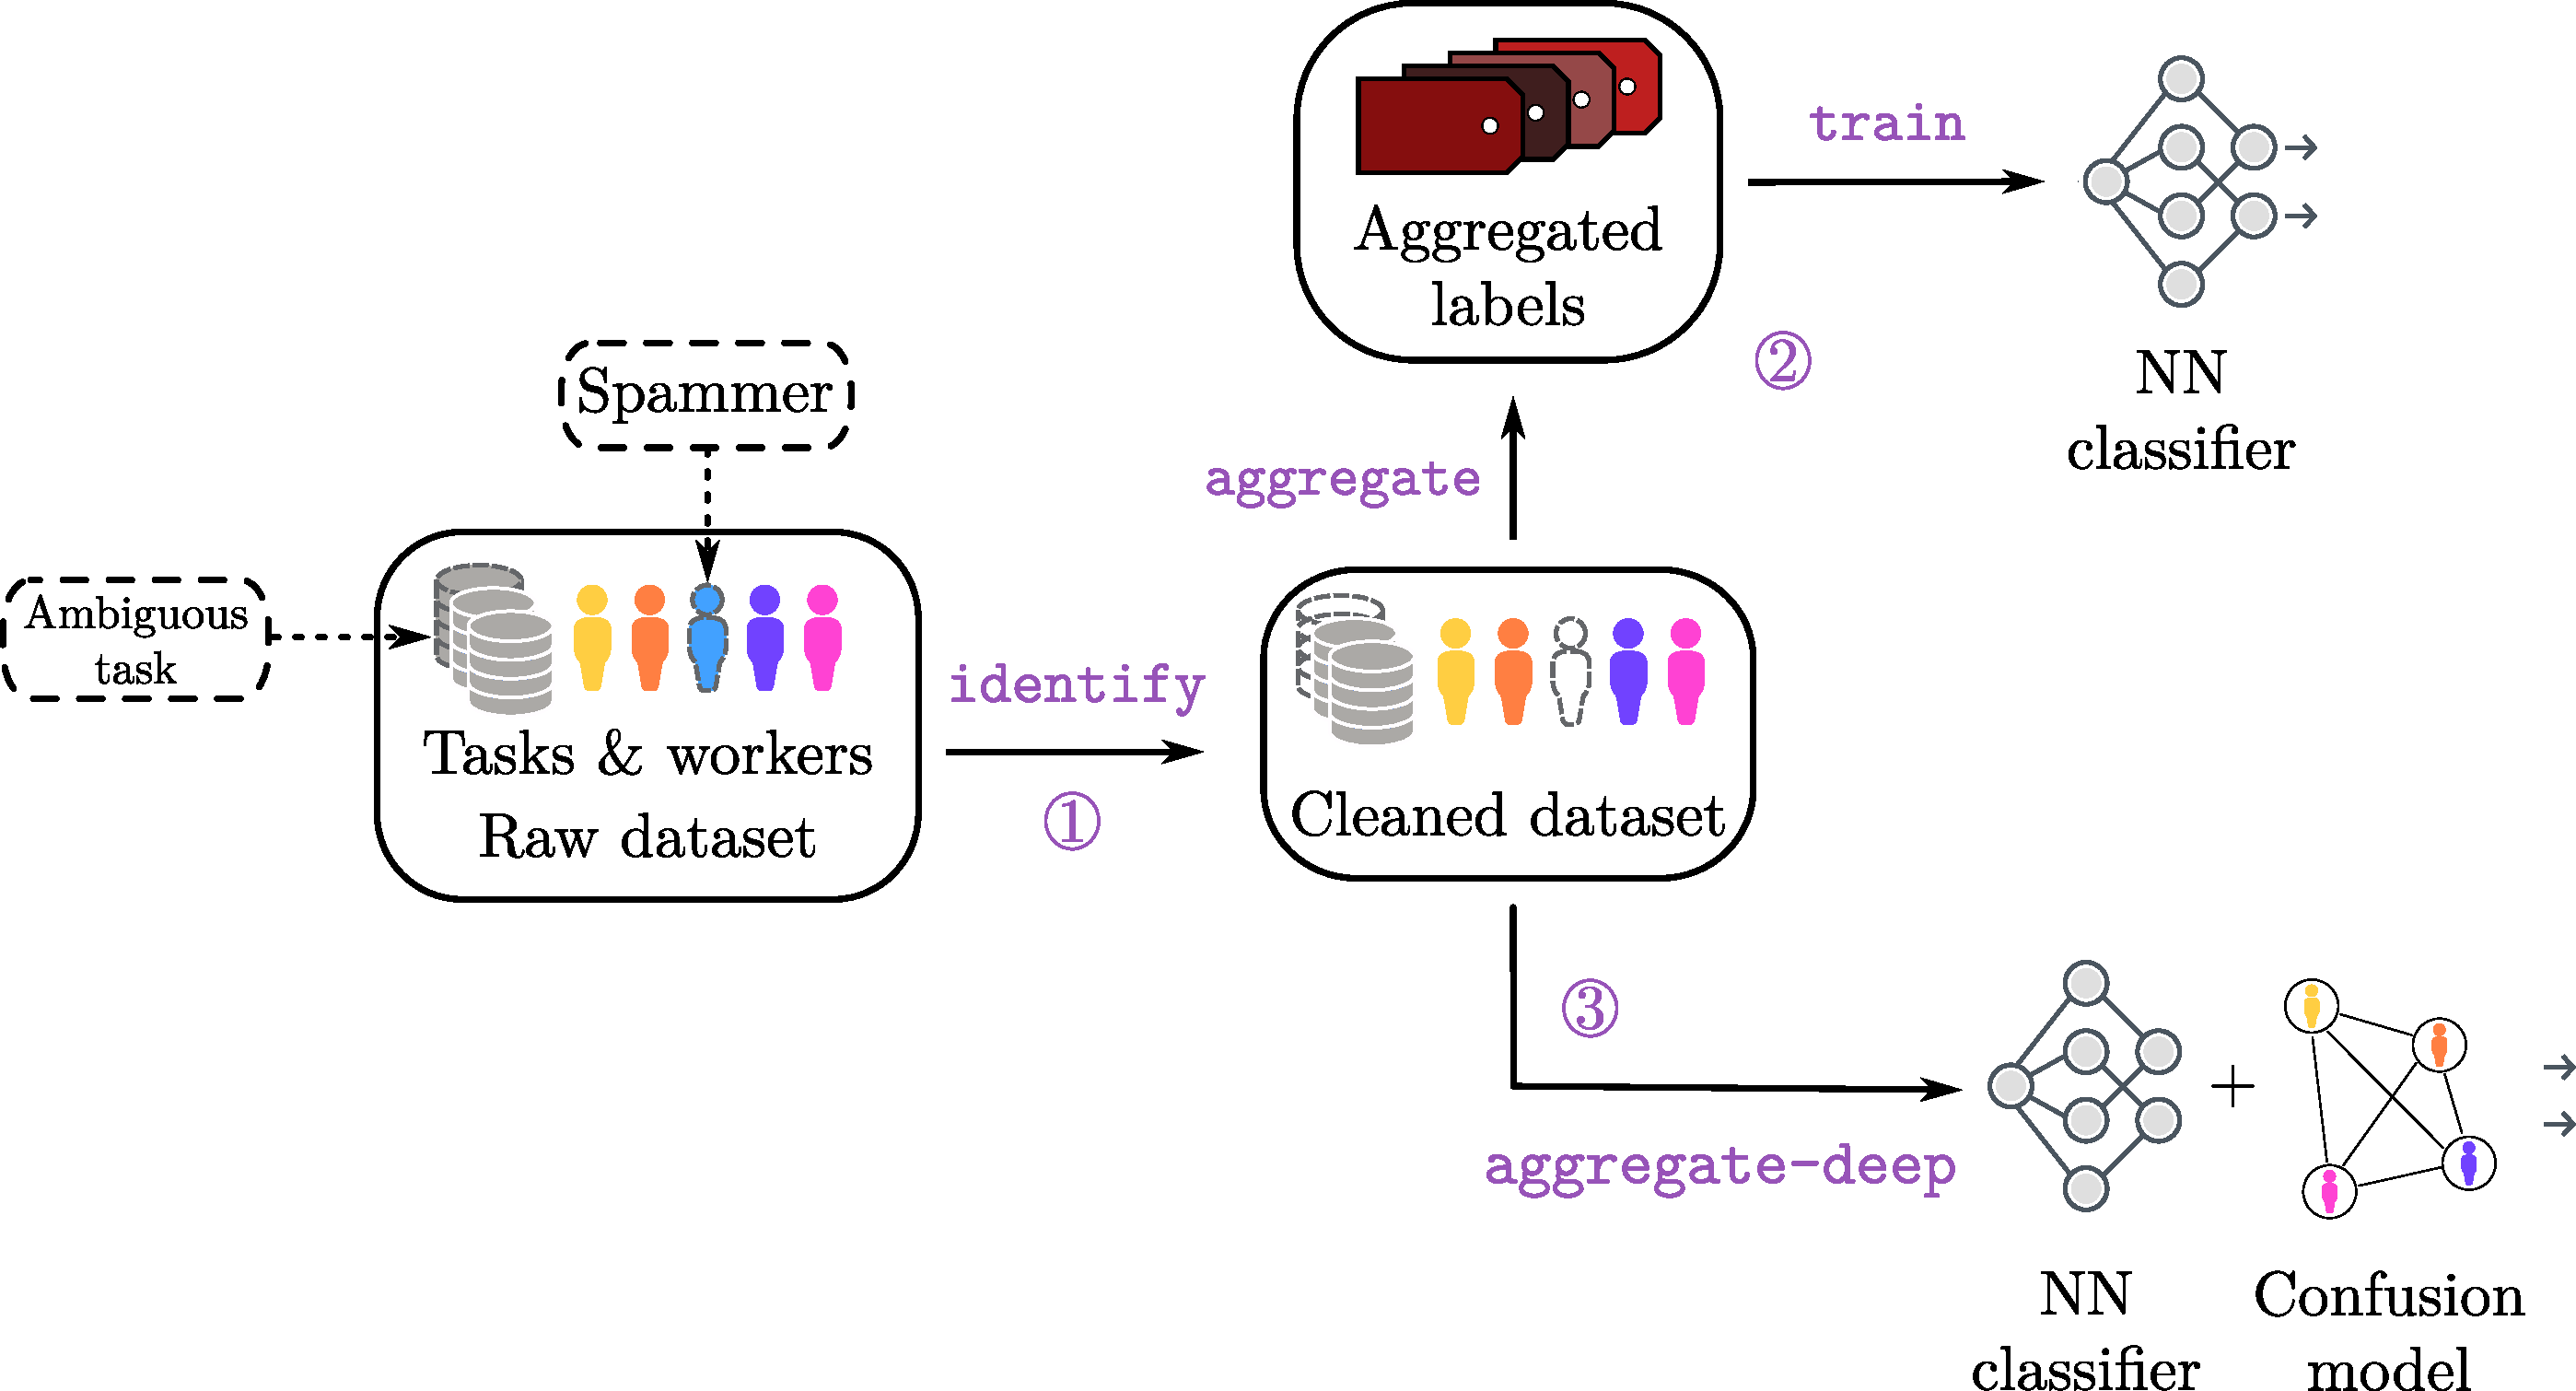
\includegraphics[width=\textwidth]{chapters/images/strategies_crowd_data.pdf}
        \caption{Pipeline on how to handle crowdsourced datasets with \texttt{peerannot}. After collecting the data, the \texttt{identify} module helps find poorly performing workers and/or ambiguous tasks. Those can be pruned to recover a \emph{cleaned} set. Then, the \texttt{aggregate} module can be used to infer a label from multiple labels. The \texttt{aggregate-deep} module can be used to train a classifier from the crowdsourced labels without aggregation. Finally, the \texttt{train} module can be used to train a classifier from aggregated labels.}
        \label{fig:pipeline_crowdsourcing_peerannot}
    \end{figure}

\subsection{Presenting the peerannot library usage}

The \texttt{peerannot} library is available on \url{https://peerannot.github.io/} and can be installed using \texttt{pip}:
\begin{minted}[linenos=true, bgcolor=lightgray, tabsize=4, fontfamily=courier, fontsize=\small, xleftmargin=5pt, xrightmargin=5pt]{bash}
$ pip install peerannot
\end{minted}

When installed, it comes with both a \texttt{python} Application Programming Interface (API) and a Command Line Interface (CLI).
Note that the \texttt{python} API is the main interface to use the library, and the CLI is a wrapper around the \texttt{python} API to make it easier to use for non-programmers.
Moreover, the CLI can be used in a \texttt{python} program in interactive cells using the \texttt{!} character to run the shell commands indicated by the dollar sign \texttt{\$}.

\subsubsection{Dataset standardization}

Crowdsourced datasets come in various forms. To store crowdsourcing datasets efficiently and in a standardized way, \texttt{peerannot} proposes the following structure, where each dataset corresponds to a folder. Let us set up a toy dataset example to understand the data structure and how to store it.

\begin{figure}[htb]
        \centering
\begin{forest}
        for tree={
            font=\ttfamily,
            grow'=0,
        %     child anchor=west,
        %     parent anchor=south,
        %     anchor=west,
            folder indent=.9em, folder icons,
        edge=densely dotted,
        % sep=10pt,
                       }
        [datasetname
            [ $\ \text{train}$
                [$\ \text{...}$]
                [$\ \text{images}$]
                [$\ \text{...}$]
            ]
            [$\ \text{val}$]
            [$\ \text{test}$]
            [metadata.json, is file]
            [answers.json, is file]
        ]
\end{forest}
\caption{Template of a dataset folder in \texttt{peerannot}. Collected votes are in \texttt{answers.json}, all necessary information on the dataset are in \texttt{metadata.json}. Tasks are either in the \texttt{train}, \texttt{val} or \texttt{test} folders. \texttt{test} tasks are assumed to have an associated ground truth label.}
\end{figure}

The \texttt{answers.json} file stores the different votes for each task as described in \Cref{fig:toy-data}. This \texttt{.json} is the rosetta stone between the task IDs and the images. It contains the tasks' id, the workers's id and the proposed label for each given vote. Furthermore, storing labels in a dictionary is more memory-friendly than having an array of size $(n_{task}, n_{worker})$ and writing $y_i^{(j)}=-1$ when the worker $w_j$ did not see the task $x_i$ and $y_i^{(j)}\in[K]$ otherwise.

\begin{figure}[htb]
\centering
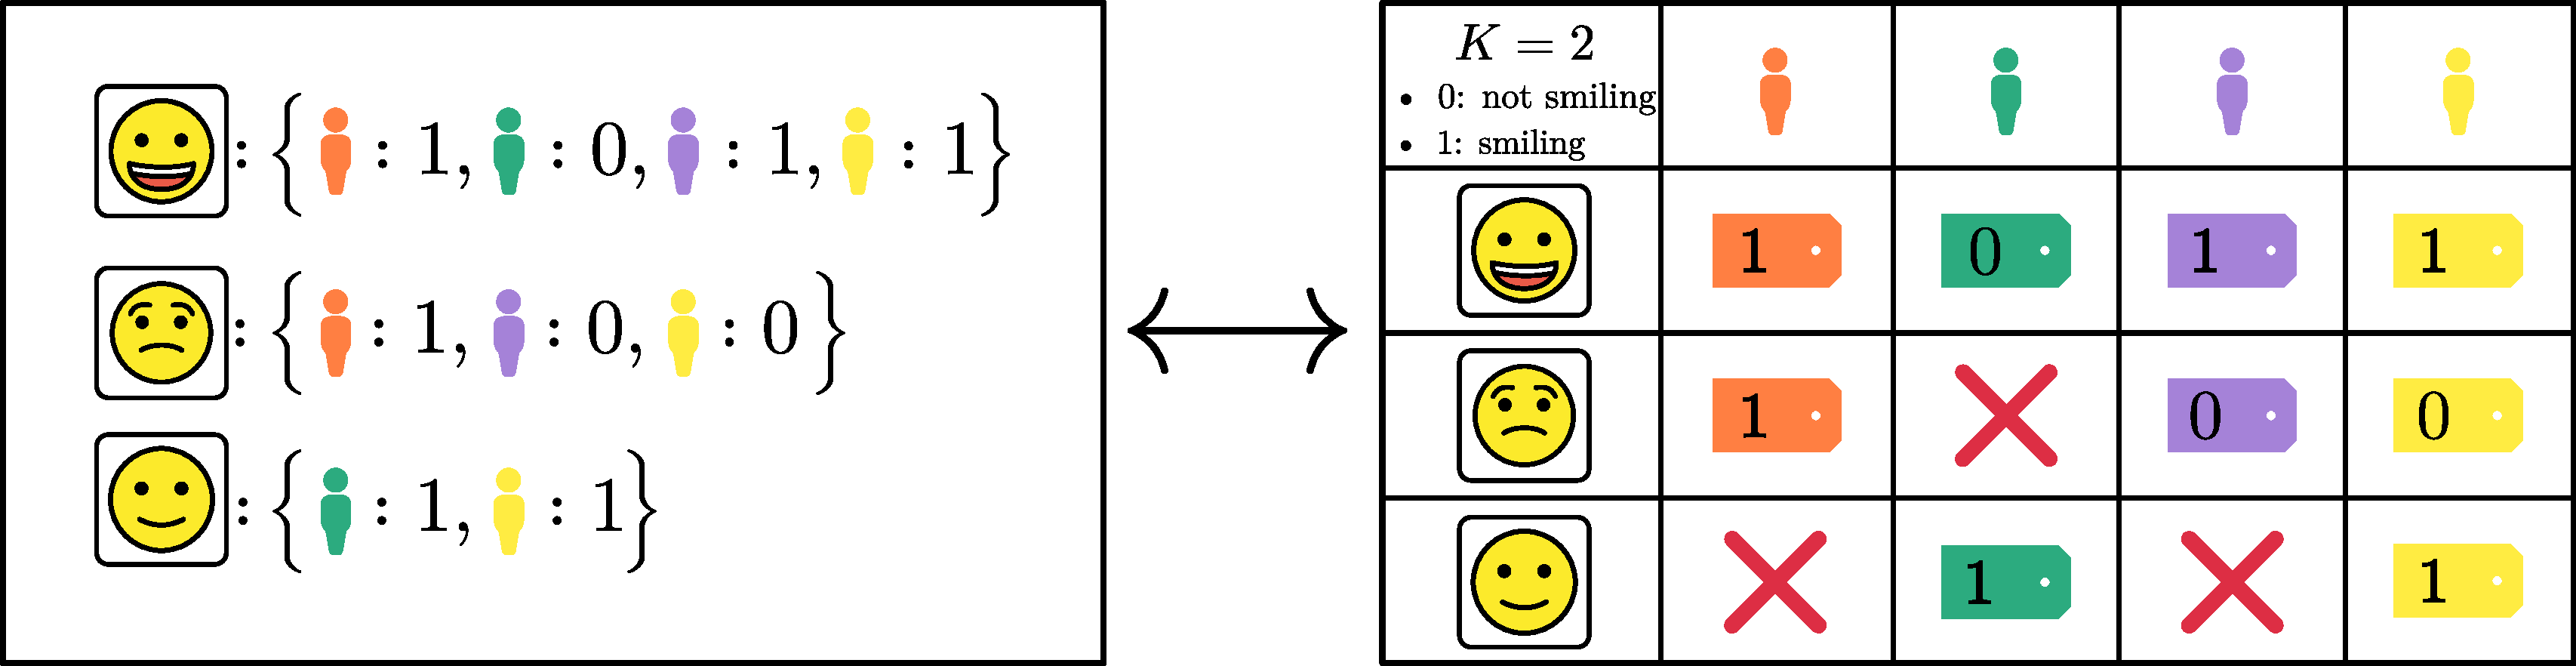
\includegraphics[width=\textwidth]{./images/json_answers.pdf}
\caption{Data storage for the \texttt{toy-data} crowdsourced dataset, a binary classification problem ($K=2$, smiling/not smiling) on recognizing smiling emoticons. On the left how \texttt{peerannot} stores the data, and on the right the raw data.}
\label{fig:toy-data}
\end{figure}

Finally, a \texttt{metadata.json} file includes relevant information related to the crowdsourcing experiment such as the number of workers, the number of tasks, \emph{etc.} For example, a minimal \texttt{metadata.json} file for the toy dataset presented in \Cref{fig:toy-data} is:
\begin{minted}[linenos=true, bgcolor=lightgray, tabsize=4, fontfamily=courier, fontsize=\small, xleftmargin=5pt, xrightmargin=5pt]{json}
{
    "name": "toy-data",
    "n_classes": 2,
    "n_workers": 4,
    "n_tasks": 3
}
\end{minted}


The toy-data example dataset is available as an example in the \texttt{peerannot} repository. Classical datasets in crowdsourcing such as \texttt{CIFAR-10H} \citep{peterson_human_2019} and \texttt{LabelMe} \citep{rodrigues2014gaussian} can be installed directly using \texttt{peerannot}. To install them, run the \texttt{install} command from \texttt{peerannot}:

\begin{minted}[linenos=true, bgcolor=lightgray, tabsize=4, fontfamily=courier, fontsize=\small, xleftmargin=5pt, xrightmargin=5pt]{bash}
$ peerannot install ./datasets/labelme/labelme.py
$ peerannot install ./datasets/cifar10H/cifar10h.py
\end{minted}

For both \texttt{CIFAR-10H} and \texttt{LabelMe}, the dataset was originally released for standard supervised learning (classification). Both datasets have been reannotated by a crowd of workers.

\subsubsection{Other popular formats}

Other popular storage formats currently exist.
For example, the \texttt{crowd-kit} library\footnote{\url{https://github.com/Toloka/crowd-kit}} uses a dataframe where each row specifies the $3$-uplet $($task, worker, label$)$.
This format is close to the \texttt{json} one, easily switchable between the two. However, it suffers from the redundancy of the task ID.
More discussion on the \texttt{crowd-kit} library is available in \Cref{sec:benchopt}.

The \texttt{LabelMe} dataset labels are stored in a dense matrix of size $(n_{\text{task}}, n_{\text{worker}})$, where each entry is the label given by the worker for the task. This format is not memory efficient for a large number of tasks or workers. Especially if workers do not get to label all tasks.

On a more practical note, the \texttt{json} format has the advantage of being easily readable and writable by humans and is also easily convertible to a data frame. It is also easy to use for \texttt{python}, \texttt{SQL} and \texttt{JavaScript}.
As large crowdsourcing web platforms use requests in \texttt{JavaScript} to send and receive data, the \texttt{json} format is a motivating choice for these applications.

\subsection{Label agggregation with \texttt{peerannot}}

In addition to the classical MV, NS, DS, GLAD aggregation strategies presented in \Cref{sub:aggregating_votes}, \texttt{peerannot} proposes a growing number of aggregation strategies to fit different needs.
The full list is available by running the command:

\begin{minted}[linenos=true, bgcolor=lightgray, tabsize=4, fontfamily=courier, fontsize=\small, xleftmargin=5pt, xrightmargin=5pt]{bash}
$ peerannot agginfo
\end{minted}


For example, the Worker Clustered DS model (DSWC) by \citet{imamura2018analysis} is based on the DS model.
Each worker belongs to one of the $L\leq n_{\text{worker}}$ clusters.
This strategy highly reduces the number of parameters.
In the original DS strategy, there are $K^2\times n_{\text{worker}}$ parameters to estimate for the confusion matrices. The DSWC strategy has $K^2\times L + L$ parameters to estimate.
Indeed, there are $L$ confusion matrices $\Lambda=\{\Lambda_1,\dots,\Lambda_L\}$ of size $K\times K$ and the confusion matrix of a cluster is assumed drawn from a multinomial distribution with weights $(\tau_1,\dots,\tau_L)\in\Delta_L$ over $\Lambda$ such that $\mathbb{P}(\pi^{(j)}=\Lambda_\ell)=\tau_\ell$ for $\ell \in [L]$.

\paragraph{Structure of a label aggregation strategy.}

All of the label aggregation strategies are stored in the \texttt{peerannot.models} module.
Each strategy is a class object in its own \texttt{python} file.
It inherits from the \texttt{CrowdModel} class template and is defined with at least three methods:
\begin{itemize}
    \item \texttt{run}(): includes the optimization procedure to obtain needed weights (\emph{e.g.} the EM algorithm for DS). It is only needed for optimization-based strategies.
    \item \texttt{get\_probas}(): returns the soft labels output for each task after running the \texttt{run} method, -- if available, otherwise it returns the hard labels.
    \item \texttt{get\_answers}(): returns the hard labels output for each task after running the \texttt{run} method.
\end{itemize}

\paragraph{Example of a label aggregation strategy.}

For example, let us consider minimal working examples (MWE) for the \texttt{NS} and the \texttt{DS} strategies.
The first in \Cref{listing:NS} is a non-parametric strategy without any optimization algorithm, and the second in \Cref{listing:DS} in \Cref{chap:app-peerannot} is an EM-based parametric strategy.

\begin{listing}[ht]
\begin{minted}[linenos=true, bgcolor=lightgray, tabsize=4, fontfamily=courier, fontsize=\small, xleftmargin=5pt, xrightmargin=5pt]{python}
from ..template import CrowdModel
import numpy as np


class NaiveSoft(CrowdModel):
    def __init__(self, answers, n_classes=2, **kwargs):
        super().__init__(answers)
        self.n_classes = n_classes

    def get_probas(self):
        baseline = np.zeros((len(self.answers), self.n_classes))
        for task_id in list(self.answers.keys()):
            task = self.answers[task_id]
            for vote in list(task.values()):
                baseline[task_id, vote] += 1
        self.baseline = baseline
        return baseline / baseline.sum(axis=1).reshape(-1, 1)

    def get_answers(self):
        return np.vectorize(self.converter.inv_labels.get)(
            np.argmax(self.get_probas(), axis=1)
        )
\end{minted}
\caption{MWE for the NS label aggregation in \texttt{peerannot}.}
\label{listing:NS}
\end{listing}

If a new user wants to add their strategy, they can follow the same structure and add it to the \texttt{peerannot} library. The strategy will then be available for all users to use through a pull request.
Then, the \texttt{Benchopt} library can access it to provide comparisons with other strategies easily shared (see \Cref{sec:benchopt}).

\subsection{Compare label aggregation strategies with simulated datasets}
\label{subsec:simulated}

Using the \texttt{peerannot} library, we can easily simulate crowdsourced answers for classification settings.
Hereafter, we present two settings: one where workers answer independently, and another where mistakes are correlated.
Another setting where the mistakes are dependent on the task's difficulty level is available in \Cref{chap:app-peerannot}.

\subsubsection{Simulated independent mistakes}

The independent mistakes setting considers that each worker $w_j$ answers follows a multinomial distribution with weights given at the row $y_i^\star$ of their confusion matrix $\pi^{(j)}\in\mathbb{R}^{K\times K}$. Each confusion row in the confusion matrix is generated uniformly in the simplex. Then, we make the matrix diagonally dominant (to represent non-adversarial workers) by switching the diagonal term with the maximum value by row. Answers are independent of one another as each matrix is generated independently and each worker answers independently of other workers. In this setting, the DS model is expected to perform better with enough data as we are simulating data from its assumed noise model.

We simulate in \Cref{lst:indep_mistakes} $n_{\text{task}}=200$ tasks and $n_{\text{worker}}=30$ workers. The number of classes is $K=5$.
Each task $x_i$ receives $|\mathcal{A}(x_i)|=10$ labels. With $200$ tasks and $30$ workers, asking for $10$ labels leads to around $\frac{200\times 10}{30}\simeq 67$ tasks per worker (with variations due to randomness in the assignations as seen in \Cref{fig:desc_independent}). Note that in practice achieving this result is not straightforward as workers can not label $67$ images without specific motivation (games, money rewards, \textit{etc.}).

\begin{listing}[H]
    \begin{minted}[linenos=true, bgcolor=lightgray, tabsize=4, fontfamily=courier, fontsize=\small, xleftmargin=5pt, xrightmargin=5pt]{bash}
$ peerannot simulate --n-worker=30 --n-task=200  --n-classes=5 \
                     --strategy independent-confusion \
                     --feedback=10 --seed 0 \
                     --folder ./simus/independent
    \end{minted}
    \caption{Simulation of independent mistakes in \texttt{peerannot}.}
    \label{lst:indep_mistakes}
\end{listing}

\begin{figure}[tbh]
    \centering
    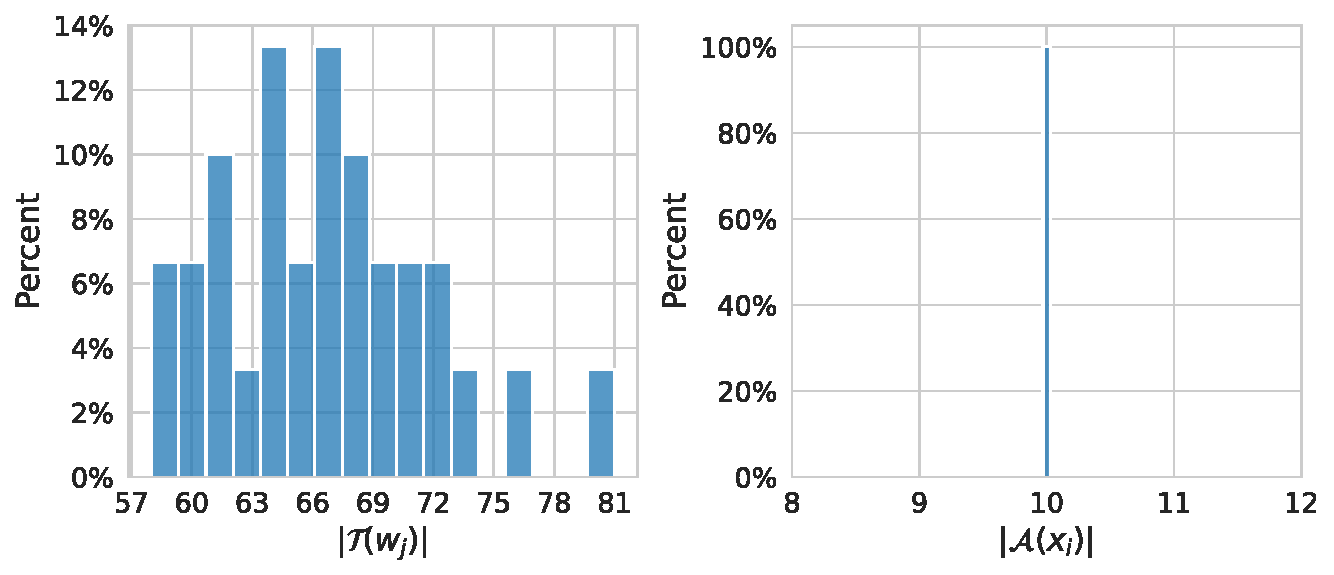
\includegraphics[width=\textwidth]{./images_peerannot/fig-simu1-output-1.pdf}
    \caption{Distribution of the number of tasks given per worker (left) and number of labels per task (right) in the independent mistakes setting.}
    \label{fig:desc_independent}
\end{figure}

With the obtained answers, we can look at the aforementioned aggregation strategies' performance. The \texttt{peerannot aggregate} command takes as input the path to the data folder and the aggregation strategy \texttt{-{}-strategy/-s}. Other arguments are available and described in the \texttt{-{}-help} description.

\begin{listing}[H]
    \begin{minted}[linenos=true, bgcolor=lightgray, tabsize=4, fontfamily=courier, fontsize=\small, xleftmargin=5pt, xrightmargin=5pt]{python}
for strat in [
    "MV", "NaiveSoft", "DS", "GLAD", "DSWC[L=5]", "DSWC[L=10]"
    ]:
  ! peerannot aggregate ./simus/independent/ -s {strat}
    \end{minted}
    \caption{Running aggregation strategies on the independent mistakes simulated dataset.}
    \label{lst:indep_mistakes_agg}
\end{listing}

\begin{table}[htbp]
    \centering
    \caption{AccTrain metric on simulated independent mistakes considering classical feature-blind label aggregation strategies.}
    \label{tab:accuracy_train_indep}
    \begin{tabular}{|l|c|c|c|c|c|c|}
    \hline
    \textbf{Strategy} & \textbf{MV} & \textbf{GLAD} & \textbf{DS} & \textbf{DSWC[L=5]} & \textbf{DSWC[L=10]} & \textbf{NS} \\
    \hline
    AccTrain & 0.765 & 0.775 & 0.890 & 0.775 & 0.770 & 0.760 \\
    \hline
    \end{tabular}
    \end{table}

As expected by the simulation framework, \Cref{tab:accuracy_train_indep} fits the DS model, thus leading to better accuracy in retrieving the simulated labels for the DS strategy. The MV and NS aggregations

\paragraph*{Remark.} \texttt{peerannot} can also simulate datasets with an imbalanced number of votes chosen uniformly at random between $1$ and the number of workers available. For example:

\begin{listing}[H]
    \begin{minted}[linenos=true, bgcolor=lightgray, tabsize=4, fontfamily=courier, fontsize=\small, xleftmargin=5pt, xrightmargin=5pt]{bash}
$ peerannot simulate --n-worker=30 --n-task=200  --n-classes=5 \
                     --strategy independent-confusion \
                     --imbalance-votes \
                     --seed 0 \
                     --folder ./simus/independent-imbalanced/
    \end{minted}
    \caption{Simulation of independent mistakes in \texttt{peerannot} with an imbalance in the number of votes per task.}
    \label{lst:indep_mistakes_simu_imb}
\end{listing}

\begin{figure}[tbh]
    \centering
    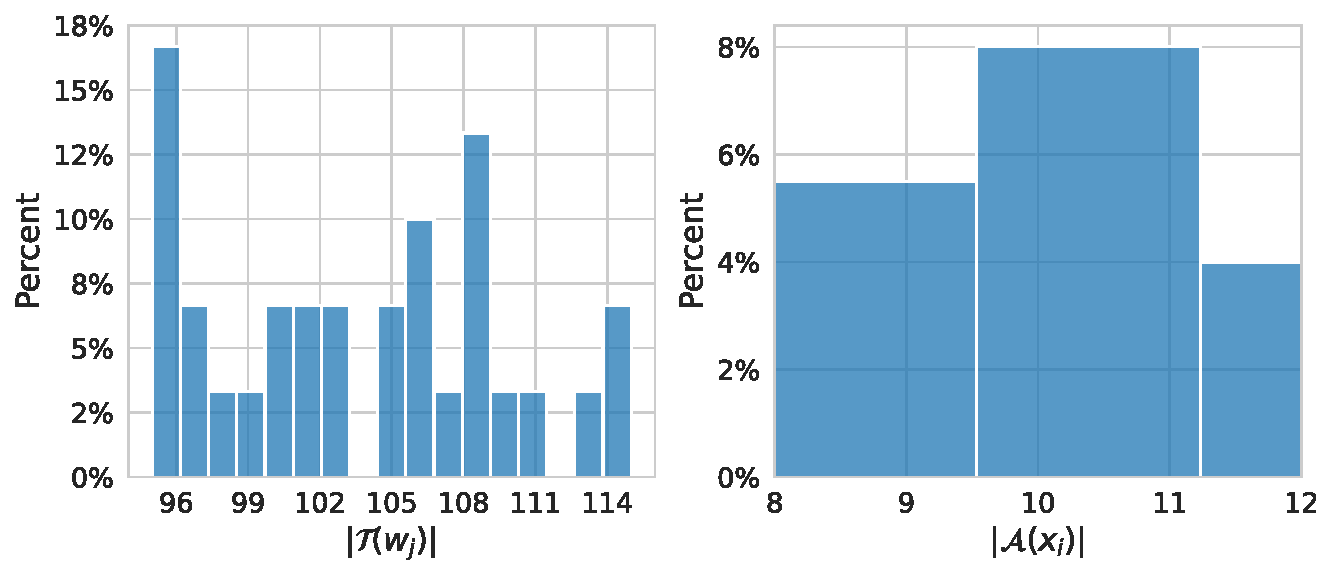
\includegraphics[width=\textwidth]{./images_peerannot/fig-simu2-output-1.pdf}
    \caption{Distribution of the number of tasks given per worker (left) and the number of labels per task (right) in the independent mistakes setting with voting imbalance enabled.}
    \label{fig:desc_independent_imbalance}
\end{figure}

With the obtained answers, we can look at the aforementioned aggregation strategies performance:

\begin{listing}[H]
    \begin{minted}[linenos=true, bgcolor=lightgray, tabsize=4, fontfamily=courier, fontsize=\small, xleftmargin=5pt, xrightmargin=5pt]{python}
for strat in [
    "MV", "NaiveSoft", "DS", "GLAD", "DSWC[L=5]", "DSWC[L=10]"
    ]:
  ! peerannot aggregate ./simus/independent-imbalanced/ -s {strat}
    \end{minted}
    \caption{Running aggregation strategies on the independent mistakes simulated dataset.}
    \label{lst:indep_mistakes_agg_imbalance}
\end{listing}

\begin{table}[htbp]
    \centering
    \caption{AccTrain metric on simulated independent mistakes, with votes imbalance, considering classical feature-blind label aggregation strategies.}
    \label{tab:accuracy_train_indep}
    \begin{tabular}{|l|c|c|c|c|c|c|}
    \hline
    \textbf{Strategy} & \textbf{MV} & \textbf{GLAD} & \textbf{DS} & \textbf{DSWC[L=5]} & \textbf{DSWC[L=10]} & \textbf{NS} \\
    \hline
    AccTrain & 0.830 &	0.810 &	0.895 	&0.845& 	0.840 &	0.830\\
    \hline
    \end{tabular}
    \end{table}

While more realistic, working with an imbalanced number of votes per task can lead to disrupting orders of performance for some strategies (here GLAD is outperformed by other strategies).

\subsubsection{Simulated correlated mistakes}
The correlated mistakes are also known as the student-teacher or junior-expert setting \citep{maxmig}. Consider that the crowd of workers is divided into two categories: teachers and students (with $n_{\text{teacher}} + n_{\text{student}}=n_{\text{worker}}$). Each student is randomly assigned to one teacher at the beginning of the experiment. We generate the confusion matrices of each teacher and the students share the same confusion matrix as their associated teacher. Hence, clustering strategies are expected to perform best in this context. Then, they all answer independently, following a multinomial distribution with weights given at the row $y_i^\star$ of their confusion matrix $\pi^{(j)}\in\mathbb{R}^{K\times K}$.

We simulate $n_{\text{task}}=200$ tasks and $n_{\text{worker}}=30$ with $80\%$ of students in the crowd. There are $K=5$ possible classes. Each task receives $\vert\mathcal{A}(x_i)\vert=10$ labels. And, with the obtained answers, we can look at the aforementioned aggregation strategies' performance:


\begin{listing}[H]
    \begin{minted}[linenos=true, bgcolor=lightgray, tabsize=4, fontfamily=courier, fontsize=\small, xleftmargin=5pt, xrightmargin=5pt]{bash}
$ peerannot simulate --n-worker=30 --n-task=200  --n-classes=5 \
                     --strategy student-teacher \
                     --ratio 0.8 \
                     --feedback=10 --seed 0 \
                     --folder ./simus/student_teacher
    \end{minted}
    \caption{Simulation of independent mistakes in \texttt{peerannot} with an imbalance in the number of votes per task.}
    \label{lst:corr_mistakes}
\end{listing}

\begin{figure}[tbh]
    \centering
    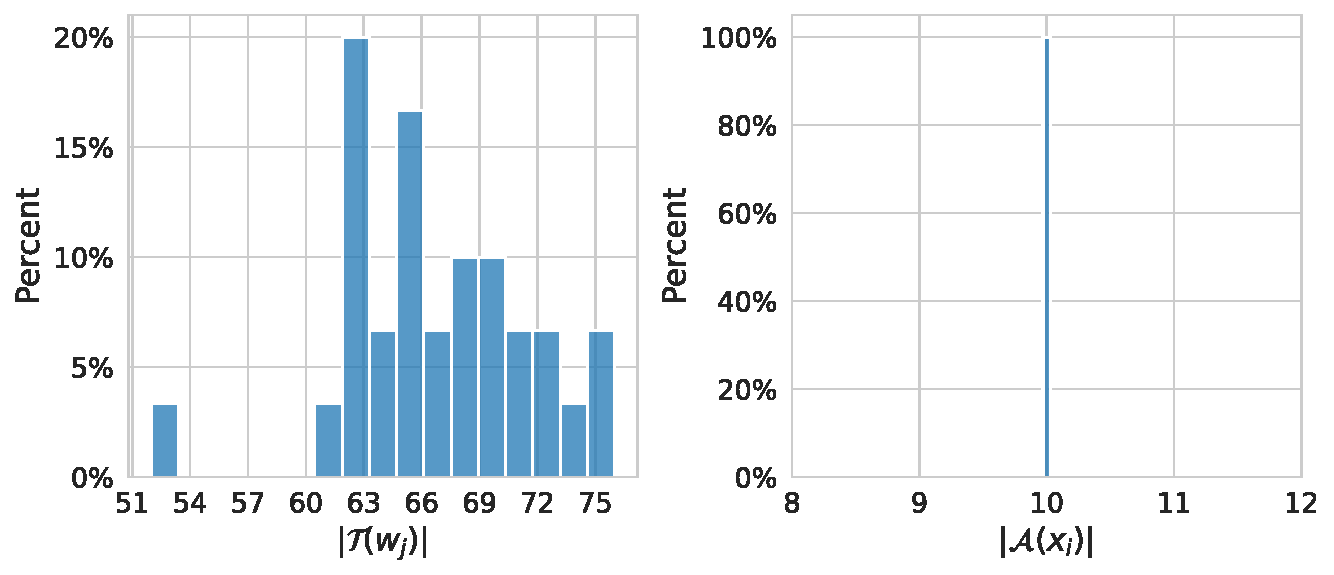
\includegraphics[width=\textwidth]{./images_peerannot/fig-simu3-output-1.pdf}
    \caption{Distribution of the number of tasks given per worker (left) and the number of labels per task (right) in the correlated mistakes setting. }
    \label{fig:desc_correlated_mistakes}
\end{figure}

\begin{table}[htbp]
    \centering
    \caption{AccTrain metric on simulated correlated mistakes considering classical feature-blind label aggregation strategies.}
    \label{tab:accuracy_train_corr}
    \begin{tabular}{|l|c|c|c|c|c|c|}
    \hline
    \textbf{Strategy} & \textbf{MV} & \textbf{GLAD} & \textbf{DS} & \textbf{DSWC[L=5]} & \textbf{DSWC[L=10]} & \textbf{NS} \\
    \hline
    AccTrain & 0.705 &	0.645 &	0.755 	&0.795 &0.815 	&0.690\\
    \hline
    \end{tabular}
    \end{table}

With \Cref{tab:accuracy_train_corr}, we see that with correlated data ($24$ students and $6$ teachers), using $5$ confusion matrices with DSWC[L=5] outperforms the vanilla DS strategy that does not consider the correlations.
The best-performing method here estimates only $10$ confusion matrices (instead of $30$ for the vanilla DS model).

To summarize our simulations, we see that depending on workers answering strategies, different latent variable models perform best.
However, these are unknown outside of a simulation framework, thus if we want to obtain labels from multiple responses, we need to investigate multiple models.
This can be done easily with \texttt{peerannot} as we demonstrated using the \texttt{aggregate} module.
However, one might not want to generate a label, simply learn a classifier to predict labels on unseen data. This leads us to another module part of \texttt{peerannot}.

\subsubsection{More on confusion matrices in simulation settings}

Moreover, the concept of confusion matrices has been commonly used to represent worker abilities.
Let us remind that a confusion matrix $\pi^{(j)}\in\mathbb{R}^{K\times K}$ of a worker $w_j$ is defined such that $\pi^{(j)}_{k,\ell} = \mathbb{P}(y_i^{(j)}=\ell\vert y_i^\star=k)$.
These quantities need to be estimated since no true label is available in a crowd-sourced scenario.
In practice, the confusion matrix of each worker is estimated via an aggregation strategy like Dawid and Skene's \citep{dawid_maximum_1979} presented in \Cref{sub:aggregating_votes}.

\begin{figure}[tbh]
    \centering
    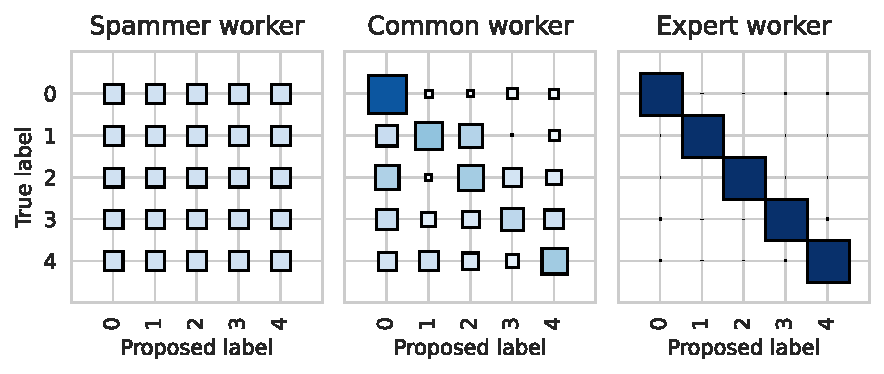
\includegraphics[width=\textwidth]{./images_peerannot/fig-confusionmatrix-output-1.pdf}
    \caption{Three types of profiles of worker confusion matrices simulated with \texttt{peerannot}. The spammer answers independently of the true label. Expert workers identify classes without mistakes. In practice common workers are good for some classes but might confuse two (or more) labels. All workers are simulated using the \texttt{peerannot simulate} command. }
    \label{fig:confusionmatrix}
\end{figure}
In \Cref{fig:confusionmatrix},  we illustrate multiple workers' profiles (as reflected by their confusion matrix) on a simulated scenario where the ground truth is available. For that, we generate toy datasets with the \texttt{simulate} command from \texttt{peerannot}.
In particular, we display a type of worker that can hurt data quality: the spammer.
\Citet{raykar_ranking_2011} defined a spammer as a worker that answers independently of the true label:
\begin{equation}\label{eq:spammer2}
    \forall k\in[K],\ \mathbb{P}(y_i^{(j)}=k|y_i^\star) = \mathbb{P}(y_i^{(j)}=k)\enspace.
\end{equation}

Each row of the confusion matrix represents the label's probability distribution given a true label. Hence, the spammer has a confusion matrix with near-identical rows -- potentially not uniform.
Apart from the spammer, common mistakes often involve workers mixing up one or several classes.
Expert workers have a confusion matrix close to the identity matrix.

\subsection{Learning from crowdsourced tasks with \texttt{peerannot}}
\label{subsec:learning_peerannot}

The \texttt{peerannot} library has also integrated end-to-end learning strategies in the \texttt{aggregate-deep} module.
Such strategies include CrowdLayer and CoNAL presented in \Cref{subsec:crowdlayer}.

Let us use \texttt{peerannot} to train a VGG-16 with two dense layers on the $\texttt{LabelMe}$ dataset. This model is called \texttt{modellabelme} in the \texttt{peerannot} library as this modification was introduced to reach state-of-the-art performance in \citet{chu2021learning}.
Other models from the \texttt{torchvision} library can be used, such as Resnets, Alexnet \emph{etc.}
The \texttt{aggregate-deep} command takes as input the path to the data folder, \texttt{-{}-output-name/-o} is the name for the output file, \texttt{-{}-n-classes/-K} the number of classes, \texttt{-{}-strategy/-s} the learning strategy to perform (\emph{e.g.}, CrowdLayer or CoNAL), the backbone classifier in \texttt{-{}-model} and then optimization hyperparameters for pytorch described with more details using the \texttt{peerannot aggregate-deep -{}-help} command as shown in \Cref{lst:learning_peerannot}.

\begin{listing}[H]
    \begin{minted}[linenos=true, bgcolor=lightgray, tabsize=4, fontfamily=courier, fontsize=\small, xleftmargin=5pt, xrightmargin=5pt]{python}
for strat in ["MV", "NaiveSoft", "DS", "GLAD"]:
    !peerannot aggregate ./labelme/ -s {strat}
    !peerannot train ./labelme -o labelme_${strat} \
        -K 8 \
        --labels=./labelme/labels/labels_labelme_${strat}.npy \
        --model modellabelme \
        --n-epochs 500 \
        -m 50 -m 150 -m 250 --scheduler=multistep \
        --lr=0.01 --num-workers=8 \
        --pretrained \
        --data-augmentation \
        --optimizer=adam \
        --batch-size=32 --img-size=224 \
        --seed=1

for strat in ["CrowdLayer", "CoNAL[scale=0]", "CoNAL[scale=1e-4]"]:
    !peerannot aggregate-deep ./labelme \
        -o labelme_${strat} \
        --answers ./labelme/answers.json \
        -s ${strat} \
        --model modellabelme \
        --pretrained \
        --n-classes=8 \
        --n-epochs=500 \
        --lr=0.001 -m 300 -m 400 --scheduler=multistep \
        --batch-size=228 --img-size=224 \
        --optimizer=adam \
        --num-workers=8 \
        --data-augmentation \
        --seed=1
    \end{minted}
    \caption{Command to learn from image classification tasks with crowdsourced labels using \texttt{peerannot}. Learning from tasks can be achieved by first aggregating labels, then, training a model. Or with end-to-end strategies calling the \texttt{aggregate-deep} command.}
    \label{lst:learning_peerannot}
\end{listing}

\begin{table}[tbh]
    \centering
    \begin{tabular}{|l|c|c|}
    \hline
    \rowcolor{gray!20}
    \textbf{Strategy} & \textbf{AccTest} & \textbf{ECE} \\
    \hline
    DS & 81.061 & 0.189 \\
    MV & 85.606 & 0.143 \\
    NS & 86.448 & 0.136 \\
    CrowdLayer & 87.205 & 0.117 \\
    GLAD & 87.542 & 0.124 \\
    CoNAL[scale=0] & 88.468 & 0.115 \\
    \cellcolor{green!20}CoNAL[scale=1e-4] & \cellcolor{green!20}88.889 & \cellcolor{green!20}0.112 \\
    \hline
    \end{tabular}
    \caption{Generalization performance on LabelMe dataset depending on the learning strategy from the crowdsourced labels. The network used is a VGG-16 with two dense layers for all methods.}
    \label{tav:perf-labelme}
    \end{table}

As we can see, CoNAL strategy performs best.
In this case, it is expected behavior as CoNAL was created for the $\texttt{LabelMe}$ dataset.
However, using \texttt{peerannot} we can look into \textbf{why modeling common confusion returns better results with this dataset}.
To do so, we can explore the datasets from two points of view: worker-wise or task-wise in \Cref{subsec:exploration}.

\subsection{Identifying tasks difficulty and worker abilities}
\label{subsec:exploration}

If a dataset requires crowdsourcing to be labeled, it is because expert knowledge is long and costly to obtain. In the era of big data, where datasets are built using web scraping (or using a platform like Amazon Mechanical Turk\footnote{\url{https://www.mturk.com/}}), citizen science is popular as it is an easy way to produce many labels.


However, mistakes and confusion happen during these experiments.
Sometimes involuntarily (\emph{e.g.,} because the task is too hard or the worker is unable to differentiate between two classes) and sometimes voluntarily (\emph{e.g.,} the worker is a spammer).

Underlying all the learning models and aggregation strategies, the cornerstone of crowdsourcing is evaluating the trust we put in each worker depending on the presented task. And with the gamification of crowdsourcing \citep{plantgame2016,tinati2017investigation}, it has become essential to find scoring metrics both for workers and tasks to keep citizens in the loop so to speak.
This is the purpose of the identification module in \texttt{peerannot}.

Our test cases are both the $\texttt{CIFAR-10H}$ dataset and the $\texttt{LabelMe}$ dataset to compare the worker and task evaluation depending on the number of votes collected.
Indeed, the $\texttt{LabelMe}$ dataset has only up to three votes per task whereas $\texttt{CIFAR-10H}$ accounts for nearly fifty votes per task.

\subsubsection{Exploring tasks' difficulty}
To explore the tasks' intrinsic difficulty, we propose to compare three scoring metrics:

\begin{itemize}
    \item the entropy of the NS distribution: the entropy measures the inherent uncertainty of the distribution to the possible outcomes. It is reliable with a big enough and not adversarial crowd. More formally:
    $$
    \forall i\in [n_{\text{task}}],\ \mathrm{Entropy}(\hat{y}_i^{NS}) = -\sum_{k\in[K]} (\hat{y}_i^{NS})_k \log\left((\hat{y}_i^{NS})_k\right) \enspace.
    $$
    \item GLAD's scoring: by construction, \citet{whitehill_whose_2009} introduced a scalar coefficient to score the difficulty of a task.
    \item the Weighted Area Under the Margins (WAUM): introduced by \citet{lefort2022improve} and presented in \Cref{chap:waum}, this weighted area under the margins indicates how difficult it is for a classifier $\mathcal{C}$ to learn a task's label. This procedure is done with a budget of $T>0$ epochs. Given the crowdsourced labels and the trust we have in each worker denoted $s^{(j)}(x_i)>0$, the WAUM of a given task $x_i\in\mathcal{X}$ and a set of crowdsourced labels $\{y_i^{(j)}\}_j \in [K]^{|\mathcal{A}(x_i)|}$ is defined as:
    $$\mathrm{WAUM}(x_i) := \frac{1}{|\mathcal{A}(x_i)|}\sum_{j\in\mathcal{A}(x_i)} s^{(j)}(x_i)\left\{\frac{1}{T}\sum_{t=1}^T  \sigma(\mathcal{C}(x_i))_{y_i^{(j)}} - \sigma(\mathcal{C}(x_i))_{[2]}\right\} \enspace,
    $$
    where we remind that $\mathcal{C}(x_i)_{[2]}$ is the second largest probability output by the classifier $\mathcal{C}$ for the task $x_i$.

    The weights $s^{(j)}(x_i)$ are computed à la \citet{servajean2017crowdsourcing}:
    $$
    \forall j\in[n_\texttt{worker}], \forall i\in[n_{\text{task}}],\ s^{(j)}(x_i) = \left\langle \sigma(\mathcal{C}(x_i)), \mathrm{diag}(\pi^{(j)})\right\rangle \enspace,
    $$
    where $\hat{\pi}^{(j)}$ is the estimated confusion matrix of worker $w_j$ (by default, the estimation provided by DS).
\end{itemize}

The WAUM is a generalization of the AUM by \citet{pleiss_identifying_2020} to the crowdsourcing setting. A high WAUM indicates a high trust in the task classification by the network given the crowd labels. A low WAUM indicates difficulty for the network to classify the task into the given classes (taking into consideration the trust we have in each worker for the task considered). Where other methods only consider the labels and not directly the tasks, the WAUM directly considers the learning trajectories to identify ambiguous tasks. One pitfall of the WAUM is that it is dependent on the architecture used.

Note that each of these statistics could prove useful in different contexts.
The entropy is irrelevant in settings with few labels per task (small $|\mathcal{A}(x_i)|$). For instance, it is uninformative for the $\texttt{LabelMe}$ dataset.
The WAUM can handle any number of labels, but the larger the better. However, as it uses a deep learning classifier, the WAUM needs the tasks $(x_i)_i$ in addition to the proposed labels while the other strategies are feature-blind.

\paragraph{Results on the \texttt{CIFAR-10H} dataset.}

First, let us consider a dataset with a large number of tasks, annotations and workers: the $\texttt{CIFAR-10H}$ dataset by \citet{peterson_human_2019}.

\begin{listing}[H]
    \begin{minted}[linenos=true, bgcolor=lightgray, tabsize=4, fontfamily=courier, fontsize=\small, xleftmargin=5pt, xrightmargin=5pt]{bash}
$ peerannot identify ./datasets/cifar10H -s entropy -K 10 \
                --labels ./   datasets/cifar10H/answers.json
$ peerannot aggregate ./datasets/cifar10H/ -s GLAD
$ peerannot identify ./datasets/cifar10H/ -K 10 \
            --method WAUM \
            --labels ./datasets/cifar10H/answers.json \
            --model resnet34 \
            --n-epochs 100 --lr=0.01 --img-size=32 \
            --maxiter-DS=50 \
            --pretrained

    \end{minted}
\caption{Command to identify ambiguous tasks on the \texttt{CIFAR-10H} dataset using \texttt{peerannot}.}
\label{lst:peeranot_identify_c10h}
\end{listing}

\begin{figure}[htb]
    \centering
    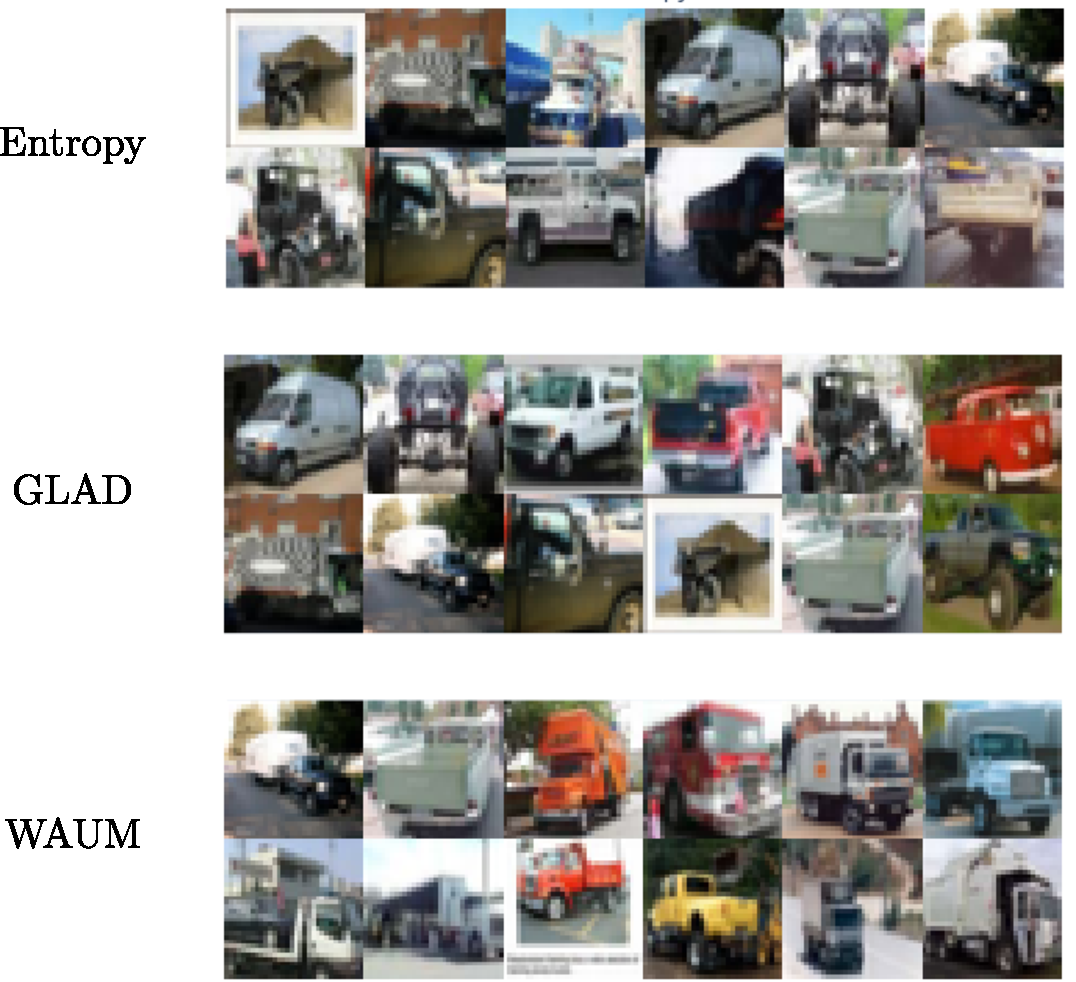
\includegraphics[width=.8\textwidth]{./images_peerannot/c10h_identification.pdf}
    \caption{Most difficult tasks sorted by class from MV aggregation identified depending on the strategy used (entropy, GLAD or WAUM) using a Resnet34. We only display the \texttt{truck} class. All class results are available interactively in the main paper at \url{https://computo.sfds.asso.fr/published-202402-lefort-peerannot/}.}
    \label{fig:identfication_c10h}
\end{figure}

The entropy, GLAD's difficulty, and WAUM's difficulty each show different images as exhibited in the interactive Figure. While the entropy and GLAD output similar tasks, in this case, the WAUM often differs. We can also observe an ambiguity induced by the labels in the \texttt{truck} category in \Cref{fig:identfication_c10h}, with the presence of a trailer that is technically a mixup between a \texttt{car} and a \texttt{truck}.

\begin{figure}[htb]
    \centering
    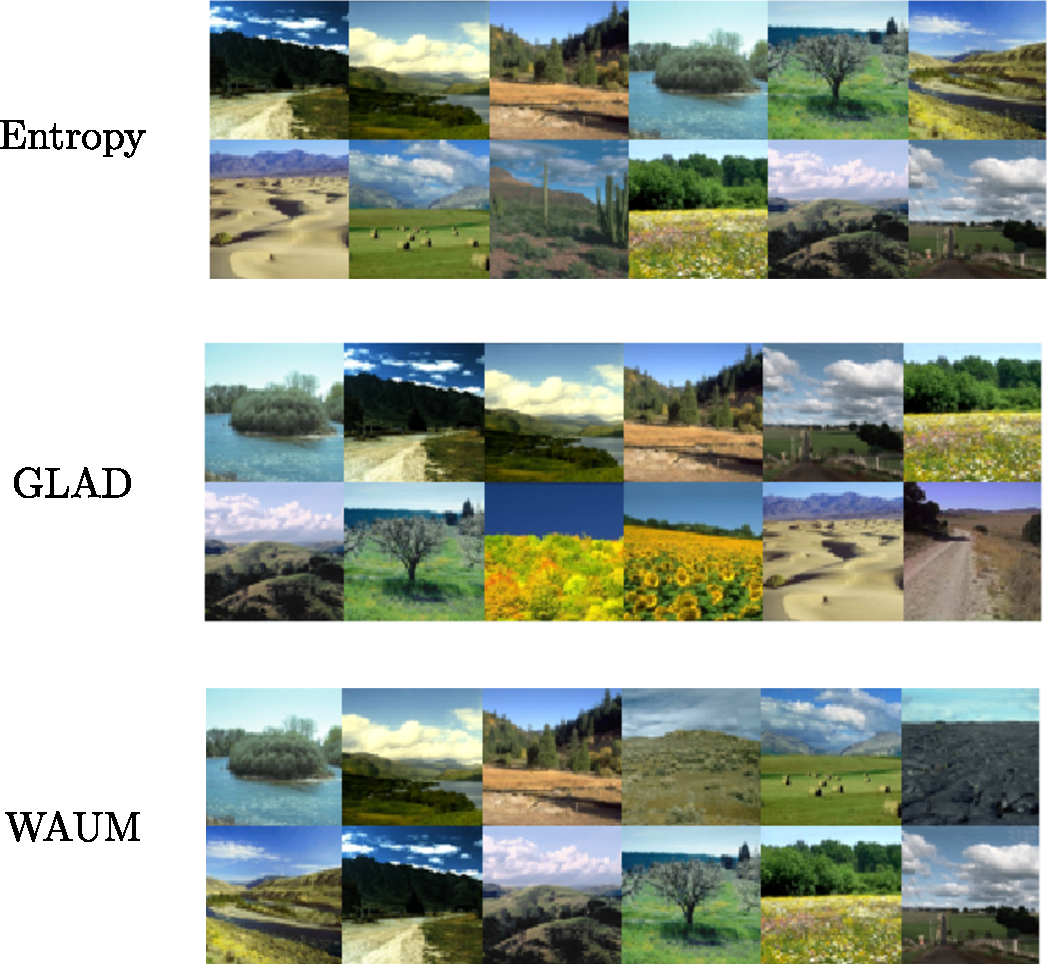
\includegraphics[width=.8\textwidth]{./images_peerannot/labelme_identification.pdf}
    \caption{Most difficult tasks sorted by class from MV aggregation identified depending on the strategy used (entropy, GLAD or WAUM) using a VGG-16 model with two dense layers. We only display the \texttt{opencountry} class. All class results are available interactively in the main paper at \url{https://computo.sfds.asso.fr/published-202402-lefort-peerannot/}.}
    \label{fig:identfication_labelme}
\end{figure}

\paragraph{Results on the \texttt{LabelMe} dataset.}

As for the $\texttt{LabelMe}$ dataset, one difficulty in evaluating tasks' intrinsic difficulty is that there is a limited amount of votes available per task.
Hence, the entropy in the distribution of the votes is no longer a reliable metric, and we need to rely on other models.

Now, let us compare the tasks' difficulty distribution depending on the strategy considered using \texttt{peerannot}.
Note that in this experiment, because the number of labels given per task is in $\{1,2,3\}$, the entropy only takes four values.
In particular, tasks with only one label all have a null entropy, so not just consensual tasks.
The MV is also not suited in this case because of the low number of votes per task.

The underlying difficulty of these tasks mainly comes from the overlap in possible labels. For example, \texttt{tallbuildings} are most often found \texttt{insidecities}, and so are \texttt{streets}. In the \texttt{opencountry} we find \texttt{forests}, river-\texttt{coasts} and \texttt{mountains}.

\subsubsection{Identification of worker reliability}

From the labels, we can explore different worker evaluation scores $s_j\in\mathbb{R}$.
GLAD's strategy estimates a reliability scalar coefficient $s_j=\alpha_j$ per worker.
With strategies looking to estimate confusion matrices, we investigate two scoring rules for workers:
\begin{itemize}
    \item The trace of the confusion matrix: the closer to $K$ the better the worker:
        \[
            \forall j\in [n_\texttt{worker}],\ s_j=\mathrm{Trace}(\pi^{(j)}) \enspace.
        \]
    \item The closeness to spammer metric \citep{raykar_ranking_2011} (also called spammer score) that is the Frobenius norm between the estimated confusion matrix $\hat{\pi}^{(j)}$ and the closest rank-$1$ matrix. Denote $\mathbf{e}$ the vector of ones in $\mathbb{R}^K$.
    \[
        \begin{aligned}
        \forall j\in [n_\texttt{worker}],\ &s_j = \|\pi^{(j)}- \mathbf{e}u_j^\top\|_F^2\enspace \\
        & \text{with } u_j = \argmin_{u\in\mathbb{R}^K, u_j\top \mathbf{e}=1} \|\pi^{(j)}- \mathbf{e}u^\top\|_F^2 \enspace.
        \end{aligned}
        \]
    Solving this problem and standardizing the result in $[0,1]$ gives the spammer score:
    \[
    \forall j \in [n_\texttt{worker}],\ s_j = \frac{1}{K(K-1)}\sum_{1\leq k<k'\leq K}\sum_{\ell\in[k]} (\pi^{(j)}_{k,\ell} - \pi^{(j)}_{k',\ell})^2 \enspace.
    \]
    The further to zero the better the worker. On the contrary, the closer to zero, the more likely it is for the worker to be a spammer. This score separates spammers from common workers and experts (with profiles as presented in \Cref{fig:confusionmatrix}).
\end{itemize}

When the tasks are available, confusion-matrix-based deep learning models can also be used.
We thus add to the comparison the trace of the confusion matrices with CrowdLayer and CoNAL on the $\texttt{LabelMe}$ datasets.
For CoNAL, we only consider the trace of the confusion matrix $\pi^{(j)}$ in the pairwise comparison.
Moreover, for CrowdLayer and CoNAL we show in \Cref{fig:abilitieslabelme} the weights learned without the softmax operation by row to keep the comparison as simple as possible with the actual outputs of the model.

Comparisons in \Cref{fig:abilitiescifarh} and \Cref{fig:abilitieslabelme} are plotted pairwise between the evaluated metrics.
Each point represents a worker.
Each off-diagonal plot shows the joint distribution between the scores of the y-axis row and the x-axis column.
They allow us to visualize the relationship between these two variables.
The main diagonal represents the (smoothed) marginal distribution of the score of the considered column.

\paragraph{Results on CIFAR-10H workers.}

The $\texttt{CIFAR-10H}$ dataset has few disagreements among workers.
However, these strategies disagree on the ranking of good against best workers as they do not measure the same properties.
We can use \texttt{peerannot} as shown in \Cref{lst:peeranot_identify_c10h_workers} to identify worker reliability on the $\texttt{CIFAR-10H}$ dataset with different strategies.

\begin{listing}[H]
    \begin{minted}[linenos=true, bgcolor=lightgray, tabsize=4, fontfamily=courier, fontsize=\small, xleftmargin=5pt, xrightmargin=5pt]{bash}
! peerannot aggregate ./datasets/cifar10H/ -s GLAD
for method in ["trace_confusion", "spam_score"]:
    ! peerannot identify ./datasets/cifar10H/ \
                    --n-classes=10 \
                    -s {method} \
                    --labels ./datasets/cifar10H/answers.json
\end{minted}
\caption{Command to identify worker reliability on the \texttt{CIFAR-10H} dataset using \texttt{peerannot}.}
\label{lst:peeranot_identify_c10h_workers}
\end{listing}

\begin{figure}[tbh]
    \centering
    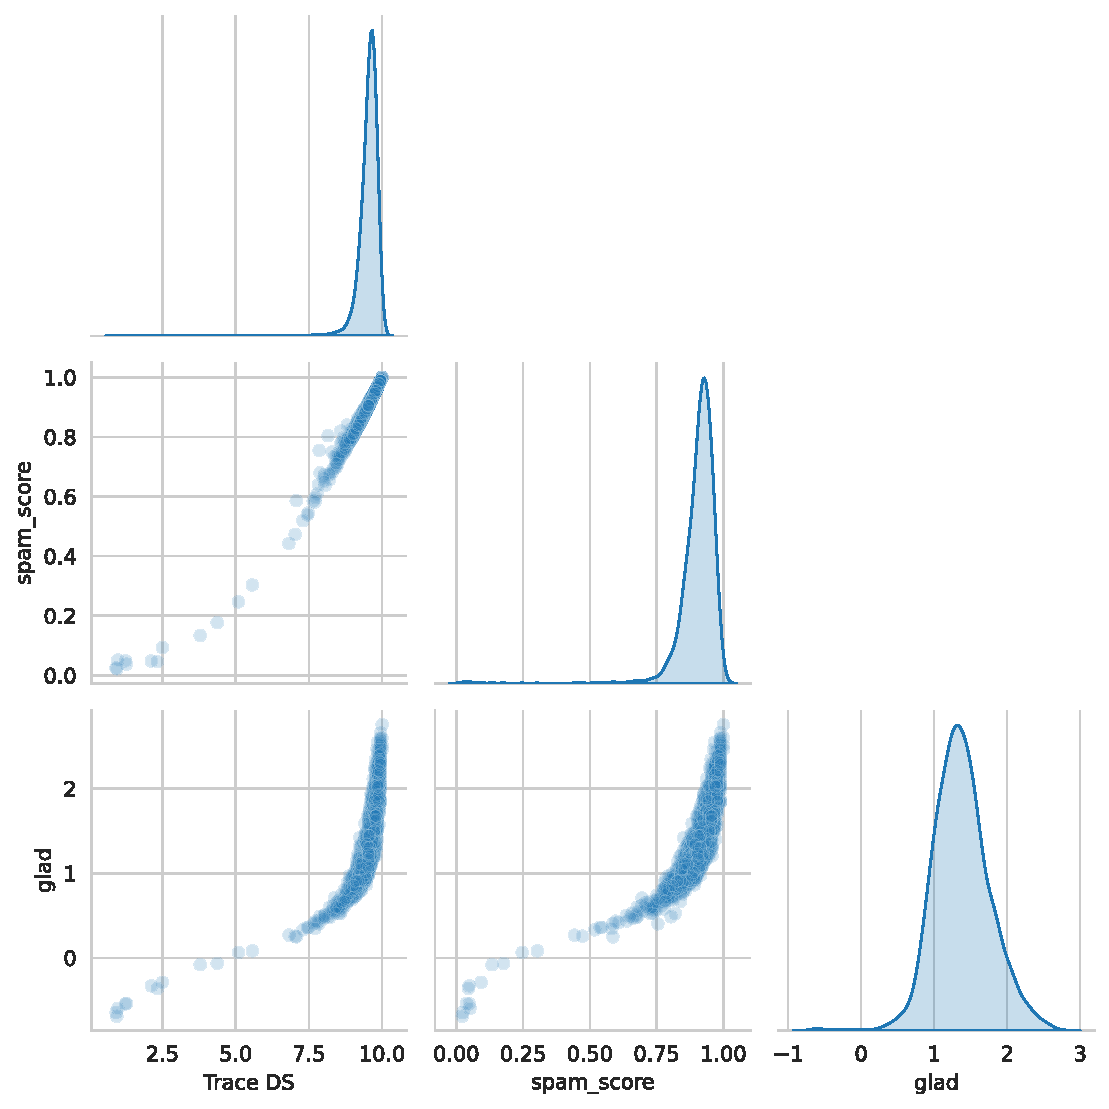
\includegraphics[width=.8\textwidth]{./images_peerannot/fig-abilitiescifarh-output-1.pdf}
    \caption{Comparison of ability scores by workers for the CIFAR-10H dataset. All metrics computed identify the same poorly performing workers. A mass of good and expert workers can be seen as the dataset presents few disagreements, thus few data to discriminate expert workers from the others.}
    \label{fig:abilitiescifarh}
\end{figure}

From \Cref{fig:abilitiescifarh}, we can see that in this dataset, different methods easily separate the worst workers from the rest of the crowd (workers in the left tail of the distribution).
Note that as different metrics investigate different properties, the best workers are not the same depending on the method used.
However, overall all strategies agree on the worst workers in this case.

\paragraph{Results on LabelMe workers.}
Finally, let us evaluate workers for the $\texttt{LabelMe}$ dataset.
Because of the lack of data (up to 3 labels per task), ranking workers is more difficult than in the $\texttt{CIFAR-10H}$ dataset.

\begin{figure}[tbh]
    \centering
    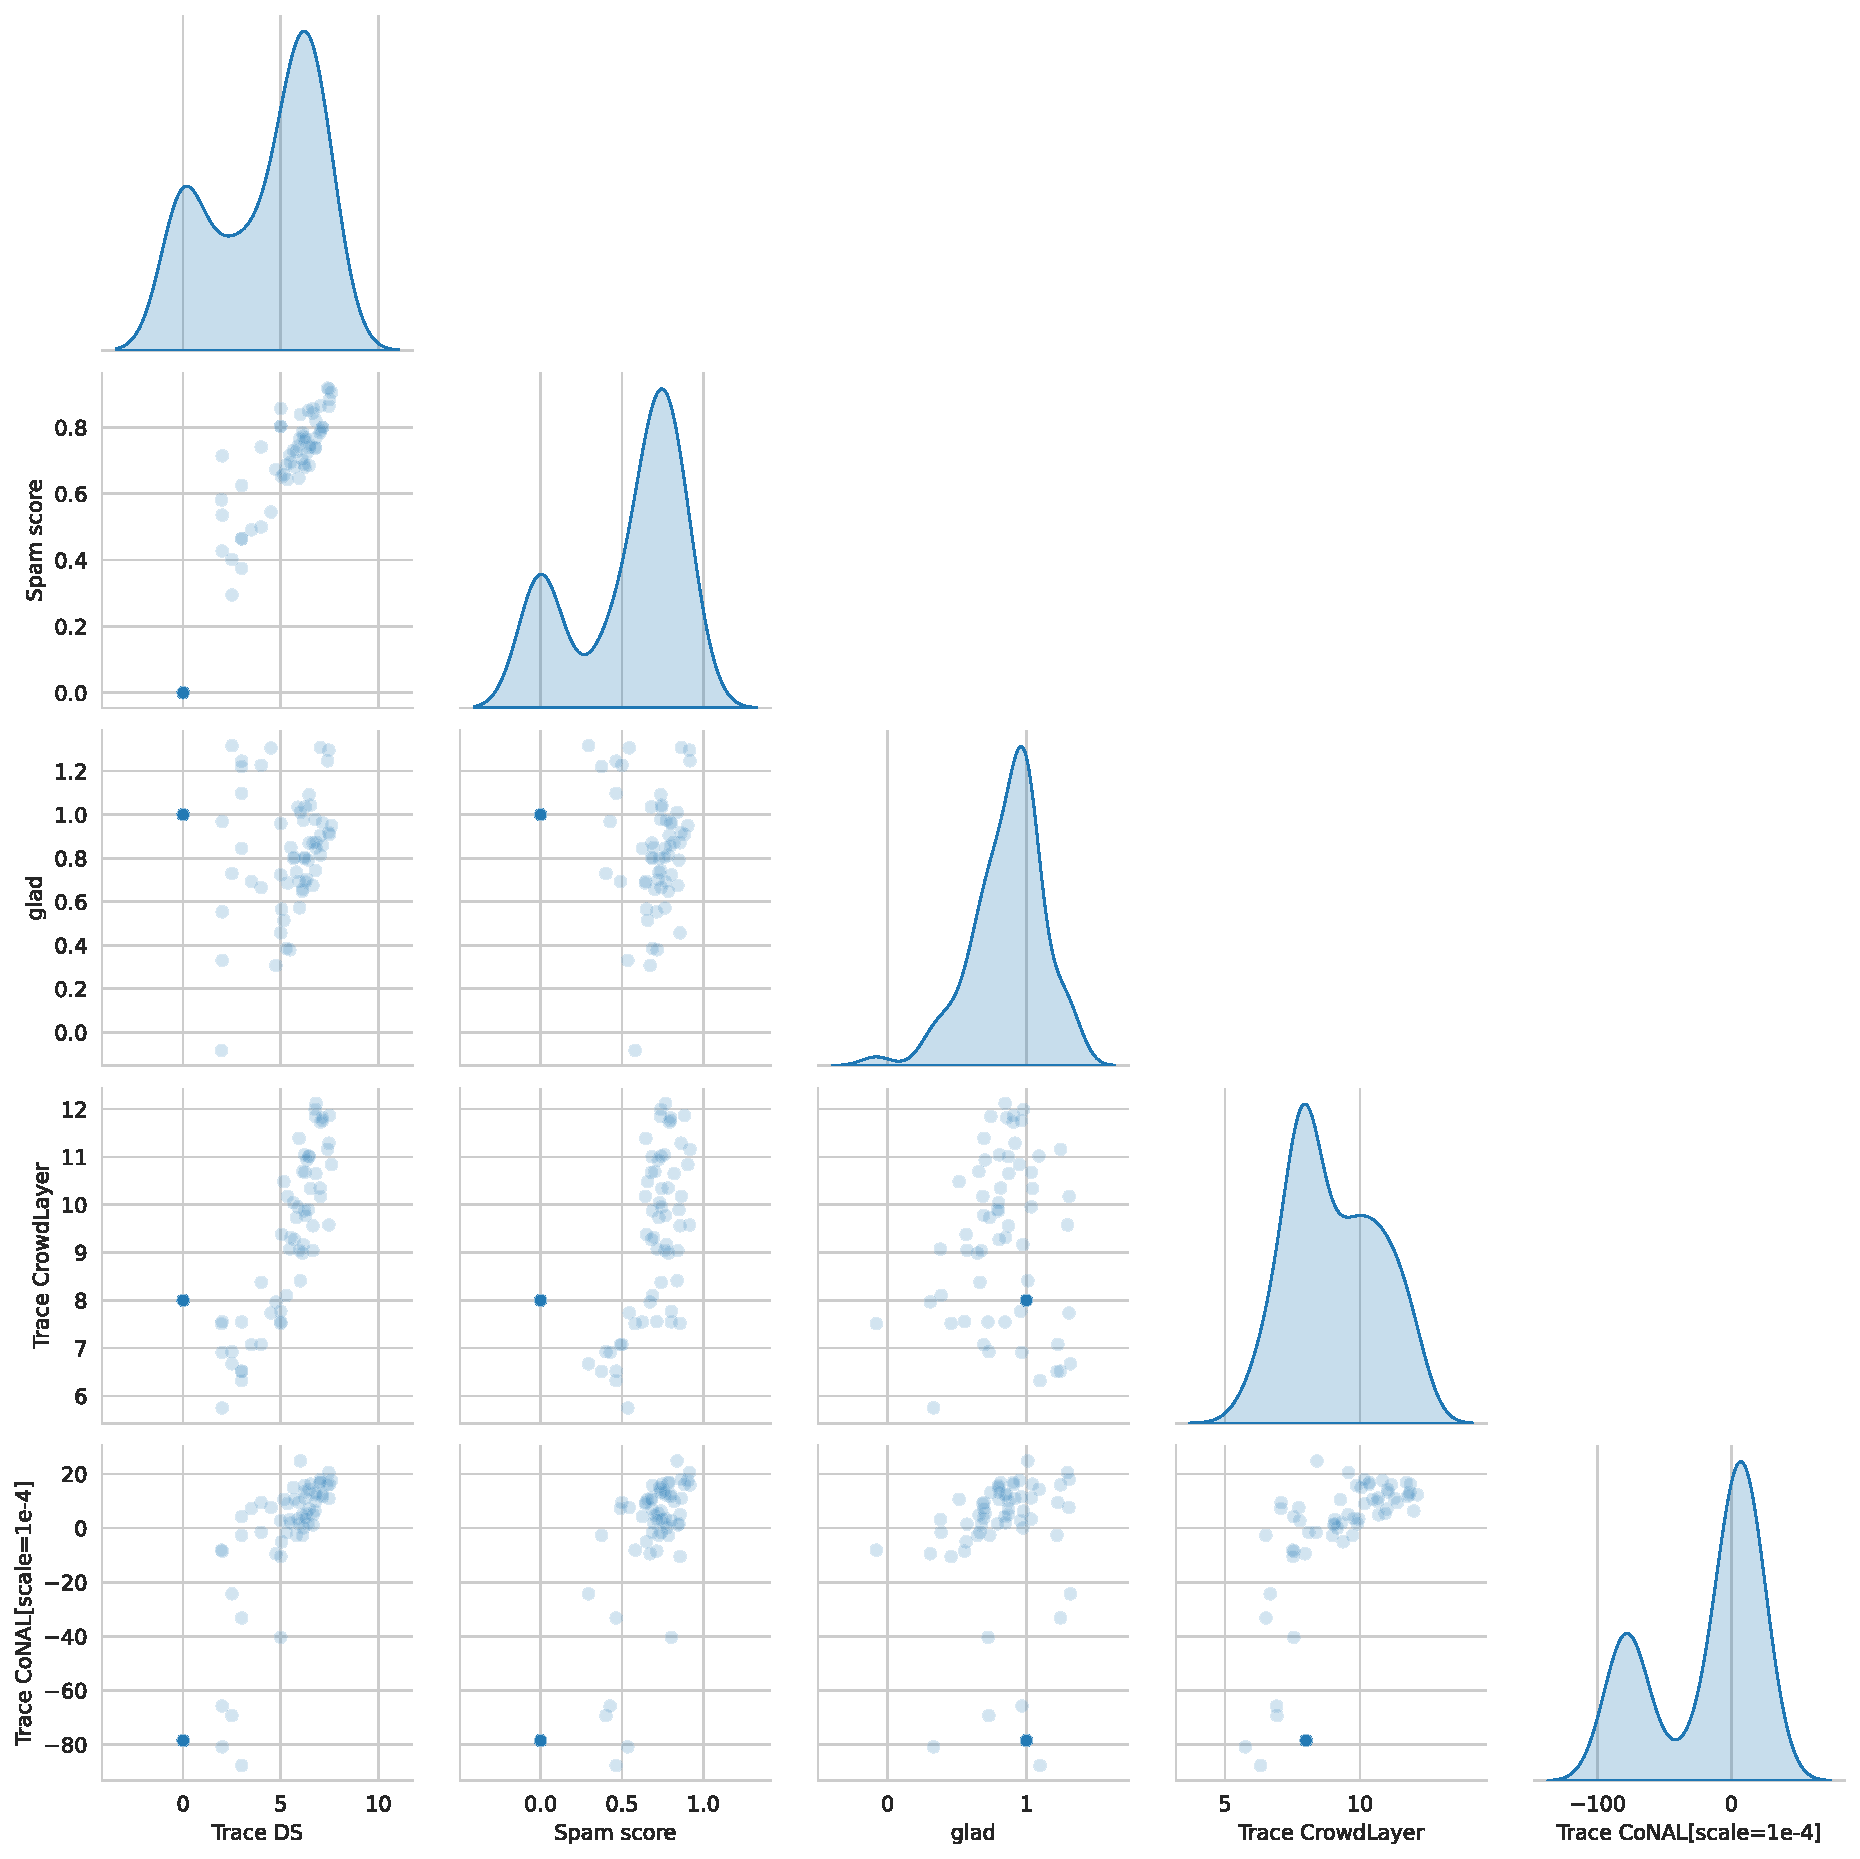
\includegraphics[width=.95\textwidth]{./images_peerannot/fig-abilities-labelme-output-1.pdf}
    \caption{With few labels per task, workers are more difficult to rank. It is more difficult to separate workers with their abilities in this crowd. Hence the importance of investigating the generalization performance of the methods presented in the previous section.}
    \label{fig:abilitieslabelme}
\end{figure}

We can see in \Cref{fig:abilitieslabelme} that the number of labels available by task highly impacts the worker evaluation scores.
The spam score, DS model and CoNAL all show similar results in the distribution shape (bimodal distribution) whereas GLAD and CrowdLayer are more concentrated.
However, this does not account for the ranking of a given worker by the methods considered.
The exploration of the dataset lets us look at different scores, but generalization performance presented in \Cref{subsec:learning_peerannot} should also be considered in crowdsourcing.
This difference in worker evaluation scores indeed further highlights the importance of using multiple test metrics to compare the model's prediction performance in crowdsourcing.
Poorly performing workers could be removed from the dataset with naive strategies like MV or NS.
However, some label aggregation strategies like DS or GLAD can sometimes use adversarial votes as information -- for example in binary classification, with a worker answering always the opposite label the confusion matrix retrieves the true label.
We have seen that the library \texttt{peerannot} allows users to explore the datasets, both in terms of tasks and of workers, and easily compare predictive performance in this setting.

In practice, the data exploration step can be used to detect possible ambiguities in the dataset's tasks, but also remove answers from spammers to improve the data quality as shown in \Cref{fig:pipeline_crowdsourcing}.
The easy access to the different strategies allows the user to decide if, for their collected dataset, there is a need for more recent deep-learning-based strategies to improve the results.
This is the case for the $\texttt{LabelMe}$ dataset.
Otherwise, the user can decide that standard aggregation-based crowdsourcing strategies are sufficient and for example, if there are plenty of votes per task like in $\texttt{CIFAR-10H}$, that the entropy of the vote distribution is a criterion that identified enough ambiguous tasks for their case.
As often, not a single strategy works best for all datasets, hence the need to perform easy comparisons with \texttt{peerannot}.

\subsection{Case study with bird sound classification}
\begin{figure}[htb]
    \centering
    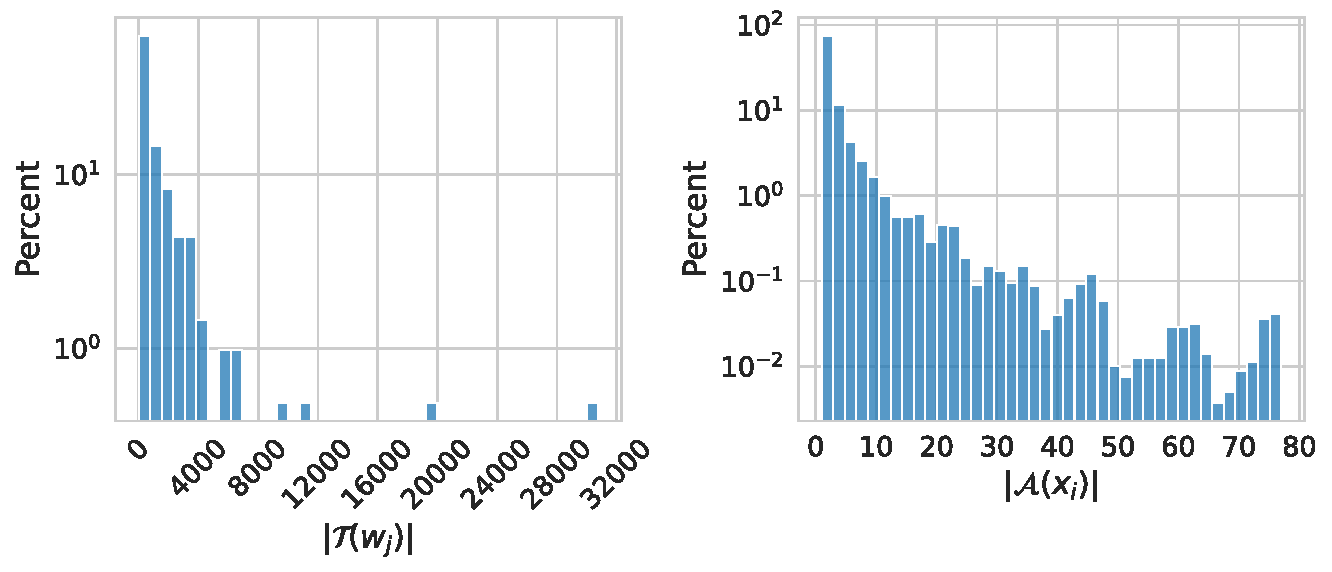
\includegraphics[width=0.95\textwidth]{./chapters/images_peerannot/fig-birdsrep-output-1.pdf}
    \caption{Distribution of the number of tasks given per worker (left) and of the number of labels per task (right) in the Audio Birds letters dataset.}
    \label{fig:birdsrep}
\end{figure}
We shared our results on the classical CIFAR-10H and LabelMe datasets.
More recently, \citet{lehikoinen2023successful} developed a platform for bird sound classification.
They released the data for the following crowdsourcing experiment.
Given the sample of the audio of a species (denoted as a letter on their web portal), users were presented with a new audio sample (the candidate).
The question is as follows: \emph{"Is the species vocalizing in the candidate the same as the species in the letter?"}
The answer is a binary yes or no ($K=2$).
In total, $n_{\text{worker}}=205$ workers labeled $n_{\text{task}}=79\, 592$ candidates.
Each task received between $1$ and $77$ annotations.
Workers answered between $1$ and $30\,759$ tasks (only one worker achieved that record, and $23\%$ of the workers answered $100$ tasks).
There is no test set available as is in the original dataset.
However, to have an idea of the level of performance of the label aggregation strategies, we use the fact that workers reported their level of expertise between $1$ and $4$.
The latter corresponds to \emph{"I am a bird researcher or professional birdwatcher"}.
This generates a test set of $13\,041$ tasks where the expert label is used as the current truth.
This test set is only used to compute the $\mathrm{AccTrain}$ metric.
Note that we do not perform deep-learning methods as the tasks of comparing the birds from two audio files and designing specific architectures to match this framework are out of the scope of this work.

We then can run our aggregation strategies, and from @tbl-birds we see that strategies reach the same levels of label recovery, however naive they are. Indeed, most tasks have very few disagreements.
Note that NS and MV performance difference comes from the random tie-breakers in case of equalities.

\begin{table}[htbp]
    \centering
    \caption{AccTrain metric on simulated correlated mistakes considering classical feature-blind label aggregation strategies.}
    \label{tab:accuracy_train_audiobirds}
    \begin{tabular}{|l|c|c|c|c|}
    \hline
    \textbf{Strategy} & \textbf{MV} & \textbf{DS} & \textbf{GLAD} & \textbf{NS} \\
    \hline
    AccTrain & 0.954 	&0.946 &	0.950& 	0.960\\
    \hline
    \end{tabular}
    \end{table}

We can explore what tasks lead to the most disagreements depending on the entropy criterion or GLAD's difficulty-estimated latent variable.
Using the entropy criterion, the most difficult tasks (highest entropy) and GLAD's difficulty, we recover the index of the most ambiguous tasks.
As we work with audio files, we can listen to the most ambiguous tasks and see if they are indeed difficult to classify.
Audio records of such identified tasks are made available at \url{https://computo.sfds.asso.fr/published-202402-lefort-peerannot/#case-study-with-bird-sound-classification}.

\begin{itemize}
    \item Entropy: we obtain the candidate \texttt{MRG18\_20180514\_000000\_203.mp3} that was to be compared with the letter \texttt{HLO15\_20180515\_021439\_31.mp3} (one worker agrees and another disagrees).
    And the candidate \texttt{MRG24\_20180512\_000000\_437.mp3} that was to be compared with the letter \texttt{HLO12\_20180511\_150153\_42.mp3} (one worker agrees and another disagrees)
    \item GLAD: we obtain the candidate \texttt{HLO04\_20180511\_034424\_15.mp3} that was to be compared with the letter \texttt{MRG11\_20180519\_000000\_506.mp3} (53 votes, 29 agreeing and 24 disagreeing). And the candidate \texttt{MRG27\_20180512\_000000\_597.mp3} that was to be compared with the letter \texttt{HLO01\_20180601\_080126\_30.mp3} (43 votes, 23 agreeing and 20 disagreeing).

\end{itemize}
In this dataset, a single task with two different votes has the highest entropy. GLAD's coefficient lets us explore tasks with multiple votes where workers were split.

We can also explore the dataset from a worker's point of view and visualize workers' performance and how many are identified as poorly performing.
This gives us an idea of the level of noise in the answers.

\begin{figure}[tbh]
    \centering
    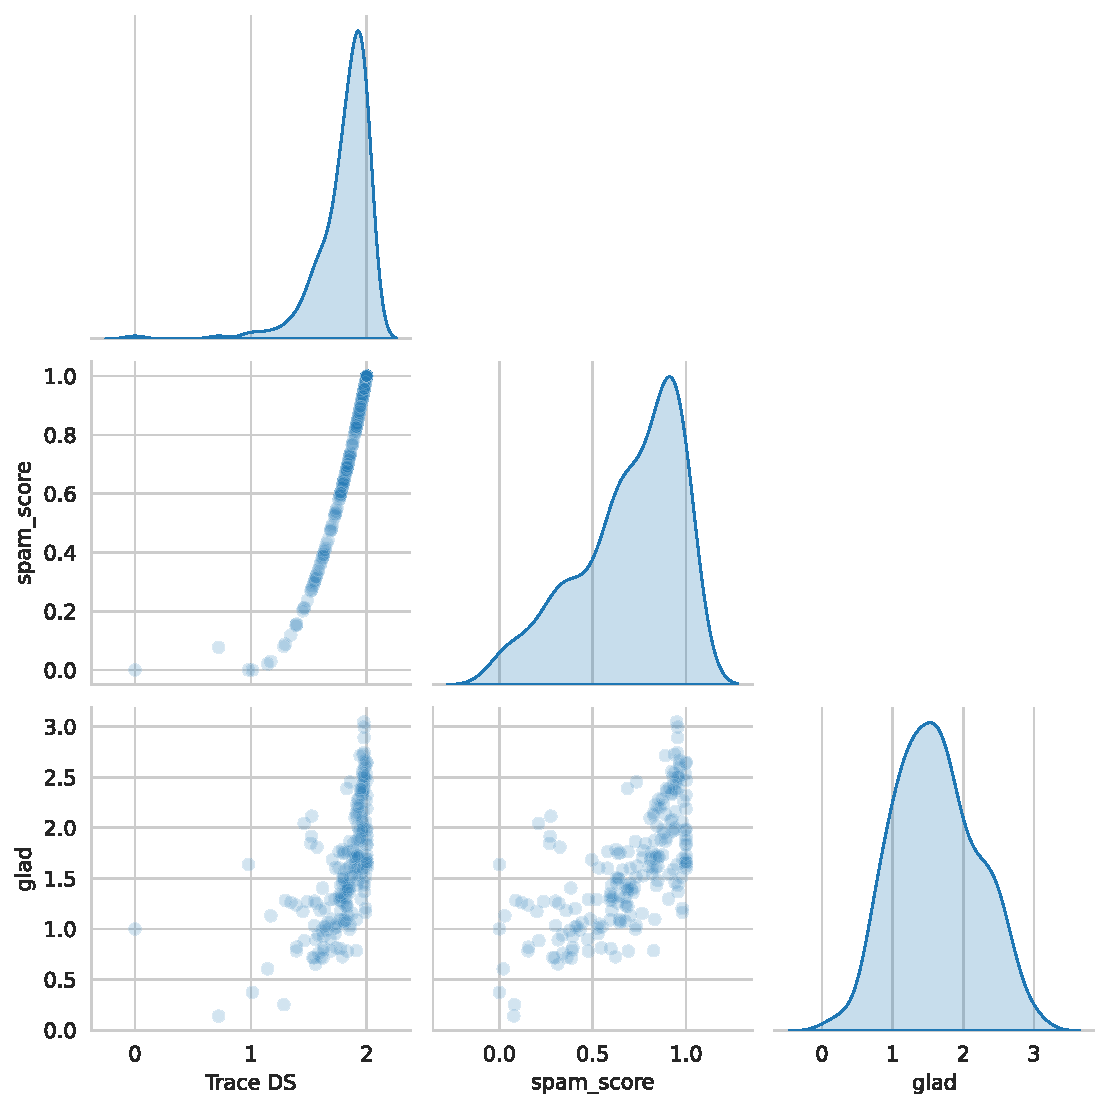
\includegraphics[width=.85\textwidth]{./images_peerannot/fig-abilitiesbird-output-1.pdf}
    \caption{Comparison of ability scores by workers for the birds audio dataset. Most workers do seem to perform similarly, with very little noise voluntarily induced.
    }
    \label{fig:abilitiesbirds}
\end{figure}

From \Cref{fig:abilitiesbirds}, we notice that very few workers are identified as spammers and that different worker identification strategies seem to perform similarly.
This is consistent with the high level of agreement between workers in this dataset.

One of the closing statements of \citet{lehikoinen2023successful} is \emph{"we learned lessons for how to better implement similar citizen science projects in the future"}.
On one hand, identifying the most ambiguous tasks can help by saving only these tasks to the most expert workers and acquiring better data.
On the other hand, combining the task difficulty with the worker ability performance metrics could help to create personal feeds of tasks to label and generate more worker participation.
Finally, the label aggregation step can lead to training classifiers with better labels.
We hope that allowing easy access thanks to the \texttt{peerannot} library to each of those steps can indeed help to better implement citizen science projects and use the collected data.

\subsection{Conclusion on \texttt{peerannot}}
We introduced \texttt{peerannot}, a library to handle crowdsourced datasets. This library enables both easy label aggregation and direct training strategies with classical state-of-the-art classifiers. The identification module of the library allows exploring the collected data from both the tasks and the workers' point of view for better scorings and data cleaning procedures.
Our library also comes with templated datasets to better share crowdsourced datasets.
Going beyond templating, it helps the crowdsourcing community to have openly accessible strategies to test, compare and improve to develop common strategies to analyze more and more common crowdsourced datasets.

We hope that this library helps reproducibility in the crowdsourcing community and also standardizes training from crowdsourced datasets. New strategies can easily be incorporated into the open-source code available on GitHub\footnote{\url{https://github.com/peerannot/peerannot}}. Finally, as \texttt{peerannot} is mostly directed to handle classification datasets, one of our future works would be to consider other \texttt{peerannot} modules to handle crowdsourcing for object detection, segmentation and even worker evaluation in other contexts like peer-grading.

\section{Benchmarking aggregation strategies with \texttt{Benchopt}}
\label{sec:benchopt}

The \texttt{Benchopt} library is an open-source benchmarking tool for optimization algorithms.
It is designed to provide a fair comparison of optimization algorithms on a wide range of problems.
The machine learning community has created platforms to release datasets (\texttt{OpenML} \citep{OpenML2013} or \texttt{DataHub}\footnote{\url{https://datahub.io/}}), reproducibility challenges \footnote{\url{https://reproml.org/}} and journals (like Rescience\footnote{\url{https://rescience.github.io/}} or Computo\footnote{\url{https://computo.sfds.asso.fr}}) to counteract the reproducibility crisis \citep{baker2016reproducibility}.
However, the optimization community has not yet developed a standard benchmarking tool to compare optimization algorithms.
This is where \texttt{Benchopt} comes in.

\subsection{How does it work?}
\label{sub:benchopt_how}

Starting from an input dataset $\mathcal{D}$ and an objective function $f$, the \texttt{Benchopt} library considers problems of the form:
\[
\argmin_{\theta\in\Theta} f(\theta, \mathcal{D},\Lambda) \enspace,
\]
where $\Lambda$ is a set of hyperparameters and $\Theta$ is the feasible set for $\theta$: the parameters in the objective.
Following the iteration sequence $\{\theta_k\}_k$ generated by an optimization algorithm, the library computes the performance of the algorithm on the problem.
Multiple objectives $f_1,f_2,\dots$ can be monitored, but only one is used in the optimization problem.

The library is designed to be modular and to allow easy integration of new optimization algorithms and new problems.
It is not \texttt{scipy}-like an optimization module with a fixed set of methods, but rather a framework to compare them on a wide range of problems, add new ones and share them.
Hardware components (number of CPUs, number of threads, GPU type, platform -- Linux version -- and libraries' version like \texttt{numpy}'s) are also stored for each benchmark.

\subsubsection{Workflow}

Each benchmark is defined by three objects. Each of them is defined as a class object in the \texttt{benchopt} library:
\begin{itemize}
    \item \textbf{Objective}: the objective function to minimize (or maximize), its hyperparameters $\Lambda$ and the set of possible parameters $\Theta$. The objective defines the performance metrics to track along the optimization sequence.
    \item \textbf{Datasets}: the data $\mathcal{D}$ to be used in the objective function. The dataset can be a simple toy dataset or a real-world dataset. It is defined separately from the objective to be modulable.
    Datasets also define how to load and preprocess the data.
    \item \textbf{Solvers}: the optimization algorithms to compare. Each solver is defined by its hyperparameters and outputs a sequence of parameters $\{\theta_k\}_k$.
\end{itemize}

\begin{figure}[htb]
    \centering
\begin{forest}
    for tree={
        font=\ttfamily,
        grow'=0,
    %     child anchor=west,
    %     parent anchor=south,
    %     anchor=west,
        folder indent=.9em, folder icons,
    edge=densely dotted,
    % sep=10pt,
                   }
    [benchmark
        [ $\ \text{datasets}$
            [$\ \text{dataset1.py}$, is file]
            [$\ \text{dataset2.py}$, is file]
            [$\ \text{...}$, is file]
        ]
        [$\ \text{solvers}$
            [$\ \text{solver1.py}$, is file]
            [$\ \text{solver2.py}$, is file]
            [$\ \text{...}$]
        ]
        [objective.py, is file]
    ]
\end{forest}
\caption{Template of a benchmark folder in \texttt{Benchopt}.}
\end{figure}

Datasets, solvers and objectives are compatible with hyperparameter settings. Solvers can have step sizes. Datasets can come with different versions or, in the case of simulations, different noise levels. Objectives can have different regularizations \emph{etc.}
Then, for each combination of dataset, solver and objective, the library computes the performance of the solver on the objective using the dataset.
These metrics are stored in a \texttt{parquet} file -- similar to a \texttt{csv} -- and then produce interactive figures using \texttt{plotly}. The full pipeline is described in \Cref{fig:benchopt}.

\begin{figure}[tbh]
    \centering
    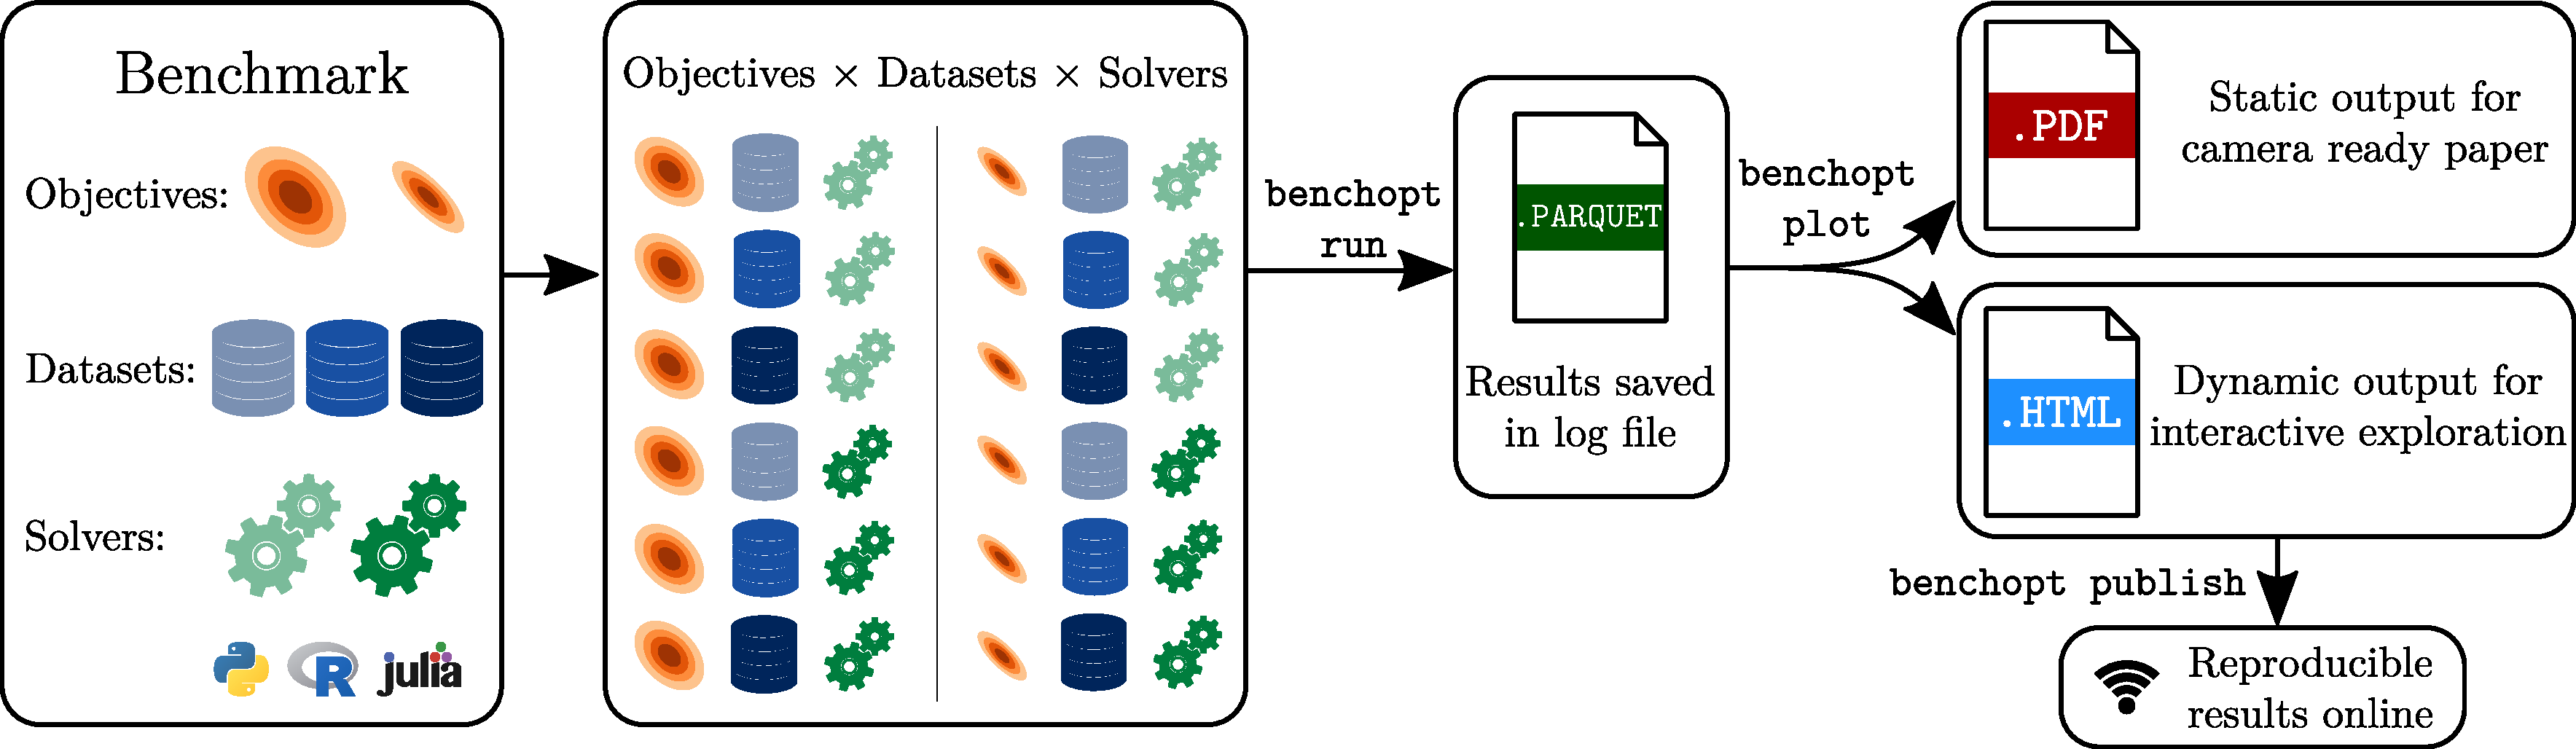
\includegraphics[width=.95\textwidth]{./images_benchopt/benchopt_schema_objectives_with_logos.pdf}
    \caption{Example of a benchmarking result with \texttt{Benchopt}. The library allows to compare the performance of different solvers on a given objective function. Results are stored in a \texttt{parquet} file as visualized using interactive \texttt{plotly} webpage. They can also be shared with the community using the \texttt{benchopt publish} command. Solvers in \texttt{Python}, \texttt{Julia} and \texttt{R} are currently supported.}
    \label{fig:benchopt}
\end{figure}

\paragraph*{Benchmark structure and dependency relation.}

As the main goal of the library is to compare solvers on different objectives, the dependency relation between the three classes is crucial.
\begin{itemize}
    \item Datasets are instantiated with a \texttt{.get\_data()} method that returns the data $\mathcal{D}$.
    \item Objectives are instantiated with a \texttt{.get\_objective()} method that returns all objects necessary for solvers to run.
    They also have a \texttt{.set\_data()} method that takes as arguments the keys of the dictionary returned by \texttt{.get\_data()}. It specifies how the data is used to compute the objective. Finally, the \texttt{.evaluate\_result()} method computes the objective.
    \item Solvers are defined with a \texttt{.set\_objective()} method that takes as arguments the keys of the dictionary returned by \texttt{.get\_objective()}. It is the main communication between the objective and the solver. The \texttt{.run()} method computes the sequence of parameters $\{\theta_k\}_k$ following a sampling strategy and a stopping criterion (discussed hereafter). Finally, the \texttt{.get\_result()} returns the estimated solution by the solver to the objective.
\end{itemize}

\begin{figure}[htb]
    \centering
    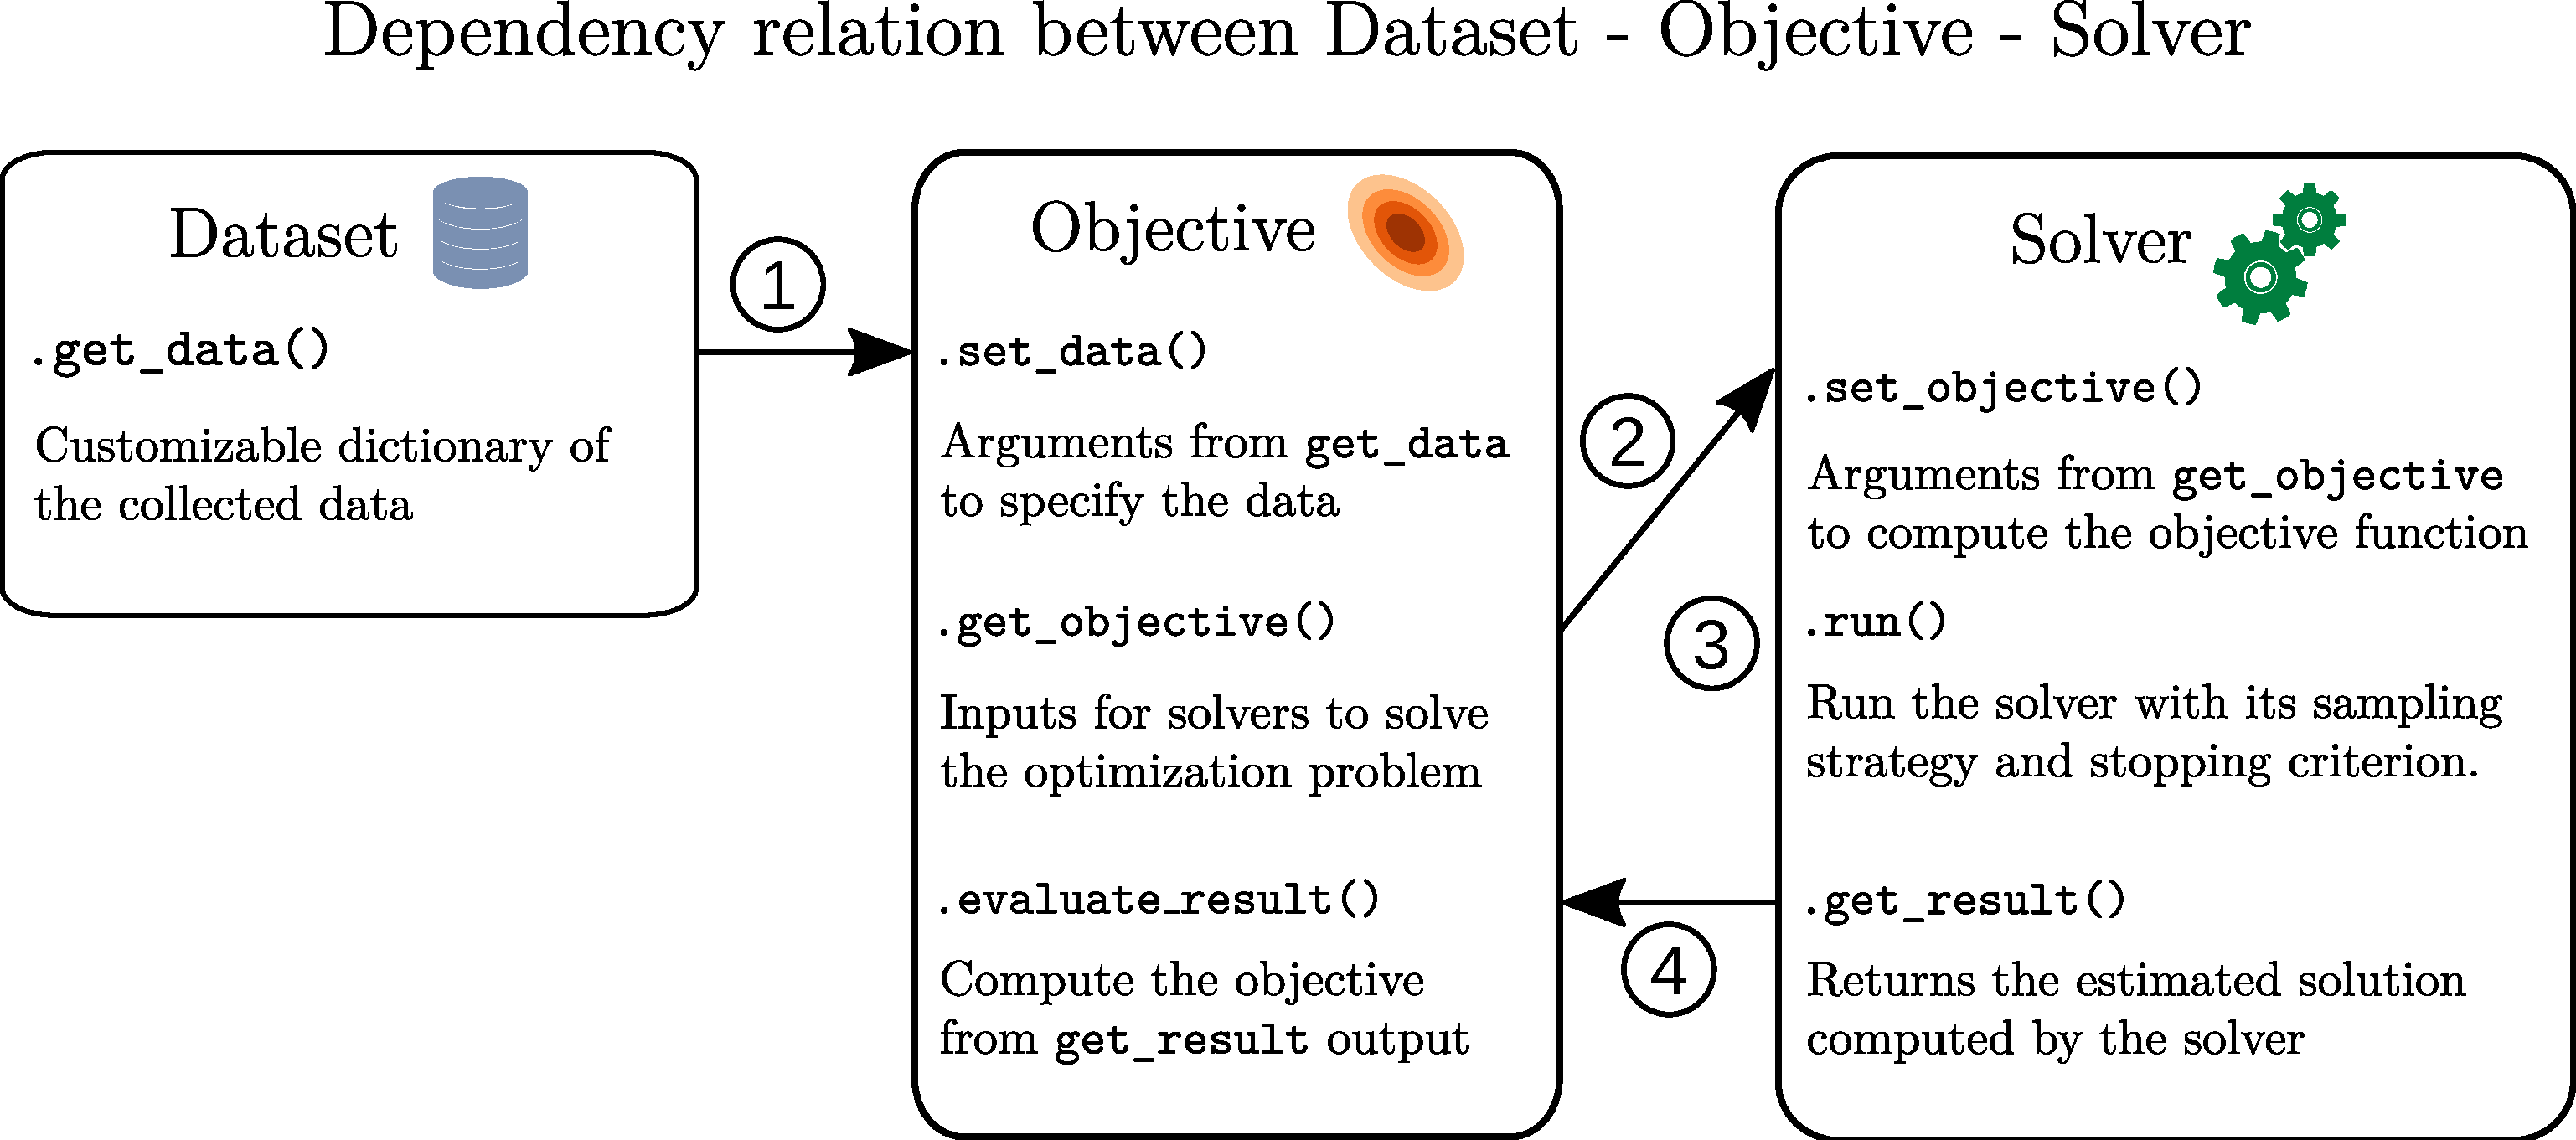
\includegraphics[width=.8\textwidth, clip, trim={0cm 0cm 0cm 1.5cm}]{./images_benchopt/benchopt_schema_dependency.pdf}
    \caption{Dependency relation between datasets, solvers and objective objects. The three classes are the core of the \texttt{Benchopt} library and communicate to run the optimization problem and monitor the performance on multiple datasets. First, the data from Datasets are passed to the Objective class. Then, the objective communicates this data for the solver to be instantiated and run. Finally, the solver returns the sequence of parameters $\{\theta_k\}_k$ to the objective to compute the performance metrics.}
    \label{fig:benchopt-dep}
\end{figure}

\subsubsection{Iterations and stopping criteria}

To evaluate each solver's performance, the library needs to define when to compute said performance during the iterative procedure.
If done for each iterate, the cost of the benchmarking procedure can be high.
Moreover, when to stop the optimization (using early stopping \citep{prechelt2002early}) in the optimization procedure is a crucial question.
Some solvers do not converge for intrinsic reasons on some datasets.
The library needs to be able to handle these cases and not let a solver run indefinitely.

\paragraph{Iterates sampling.}
The sampling for which the performance is computed is defined by the \texttt{solver.sampling\_strategy} attribute.
It can either be \texttt{"iteration"} or \texttt{"tolerance"} depending on the way the solver itself is implemented (see \Cref{fig:implementation}).

\begin{figure}[htbp]
    \centering
    \begin{minipage}[t]{0.45\textwidth}
        \begin{minted}[linenos=true, bgcolor=lightgray, tabsize=4, fontfamily=courier, fontsize=\small, xleftmargin=5pt, xrightmargin=5pt]{python}
def gd(grad, x0, lr, maxiter):
    x = x0
    for i in range(maxiter):
        # Compute gradient
        g = grad(x)
        # Update parameters
        theta -= lr * g
    return theta
        \end{minted}
        \caption*{Example of gradient descent implementation based on the number of iterations.}
    \end{minipage}
    \hfill
    \begin{minipage}[t]{0.45\textwidth}
        \begin{minted}[linenos=true, bgcolor=lightgray, tabsize=4, fontfamily=courier, fontsize=\small, xleftmargin=5pt, xrightmargin=5pt]{python}
def gd(grad, x0, lr, epsilon):
    x = x0
    norm_g = np.inf
    while norm_g > epsilon:
        # Compute gradient
        g = grad(x)
        # Update parameters
        theta -= lr * g
        # Update gradient norm
        norm_g = np.sum(g**2)
    return theta
        \end{minted}
        \caption*{Example of gradient descent implementation based on a threshold on the gradient's norm.}
    \end{minipage}
    \caption{Two examples of gradient descent implementations. The first one is based on the number of iterations and the second one on a threshold on the gradient's norm. In practice, both criteria are often combined.}
    \label{fig:implementation}
\end{figure}

\begin{itemize}
    \item iteration sampling: if the sampling strategy is set to \texttt{iteration}, the performance is computed for iterates of the solver following a geometrical growth sequence of parameter $\rho=1.5$. Starting from the first iterate, the next stopping iterate $\text{iter}_\text{stop}$ is computed as:
    \[\text{iter}_\text{stop} = \max(\text{iter}_\text{stop} + 1 , \texttt{int}(\rho \text{iter}_\text{stop})) \enspace.\]
    \item tolerance sampling: if the sampling strategy is set to \texttt{tolerance}, the performance is computed for iterates of the solver reaching a tolerance threshold. This threshold sequence follows a geometrical sequence of parameter $\rho=1.5$. Starting from $1$, the next stopping threshold $\text{thresh}_\text{stop}$ is computed when:
    \[\text{thresh}_\text{stop} = \min\left(1, \max\left(\frac{\text{iter}_\text{stop}}{\rho}, 10^{-15}\right)\right) \enspace.\]
\end{itemize}

Note that if no difference is observed between two consecutive objective calls (the variation of the objective is zero), then $\rho$ is increased by a factor of $1.2$. This is to avoid computing the same objective multiple times and obtaining a flat curve. This growth can be manually changed if needed\footnote{\url{https://benchopt.github.io/user\_guide/performance\_curves.html\#changing-the-strategy-to-grow-the-computational-budget-stop-val}}.

\paragraph{Stopping criterion.}
The stopping criterion is defined by the \texttt{solver.stopping\_criterion} attribute.
There are three possible stopping criteria and two fail-safes implemented in \texttt{Benchopt}:
\begin{itemize}
    \item Sufficient Decrease Criterion: defined by a tolerance $\varepsilon$ and a patience $p\in\mathbb{N}$. The solver is stopped when the relative decrease of the objective is less than $\varepsilon$ for $p$ evaluated samples.
    \item Sufficient Progress Criterion: defined by a tolerance $\varepsilon$ and a patience $p\in\mathbb{N}$. The solver is stopped when the objective has not decreased by more than $\varepsilon$ for $p$ evaluated samples.
    \item Single Run Criterion: the performance is evaluated only once at a given value.
\end{itemize}

The fail-safes are a maximum number of solver runs and a maximum time to run the solver. They are set to $10$ and $100$ seconds by default, respectively.

\subsection{Case study: benchmarking aggregation strategies in crowdsourcing}

\begin{figure}[htbp]
    \centering
    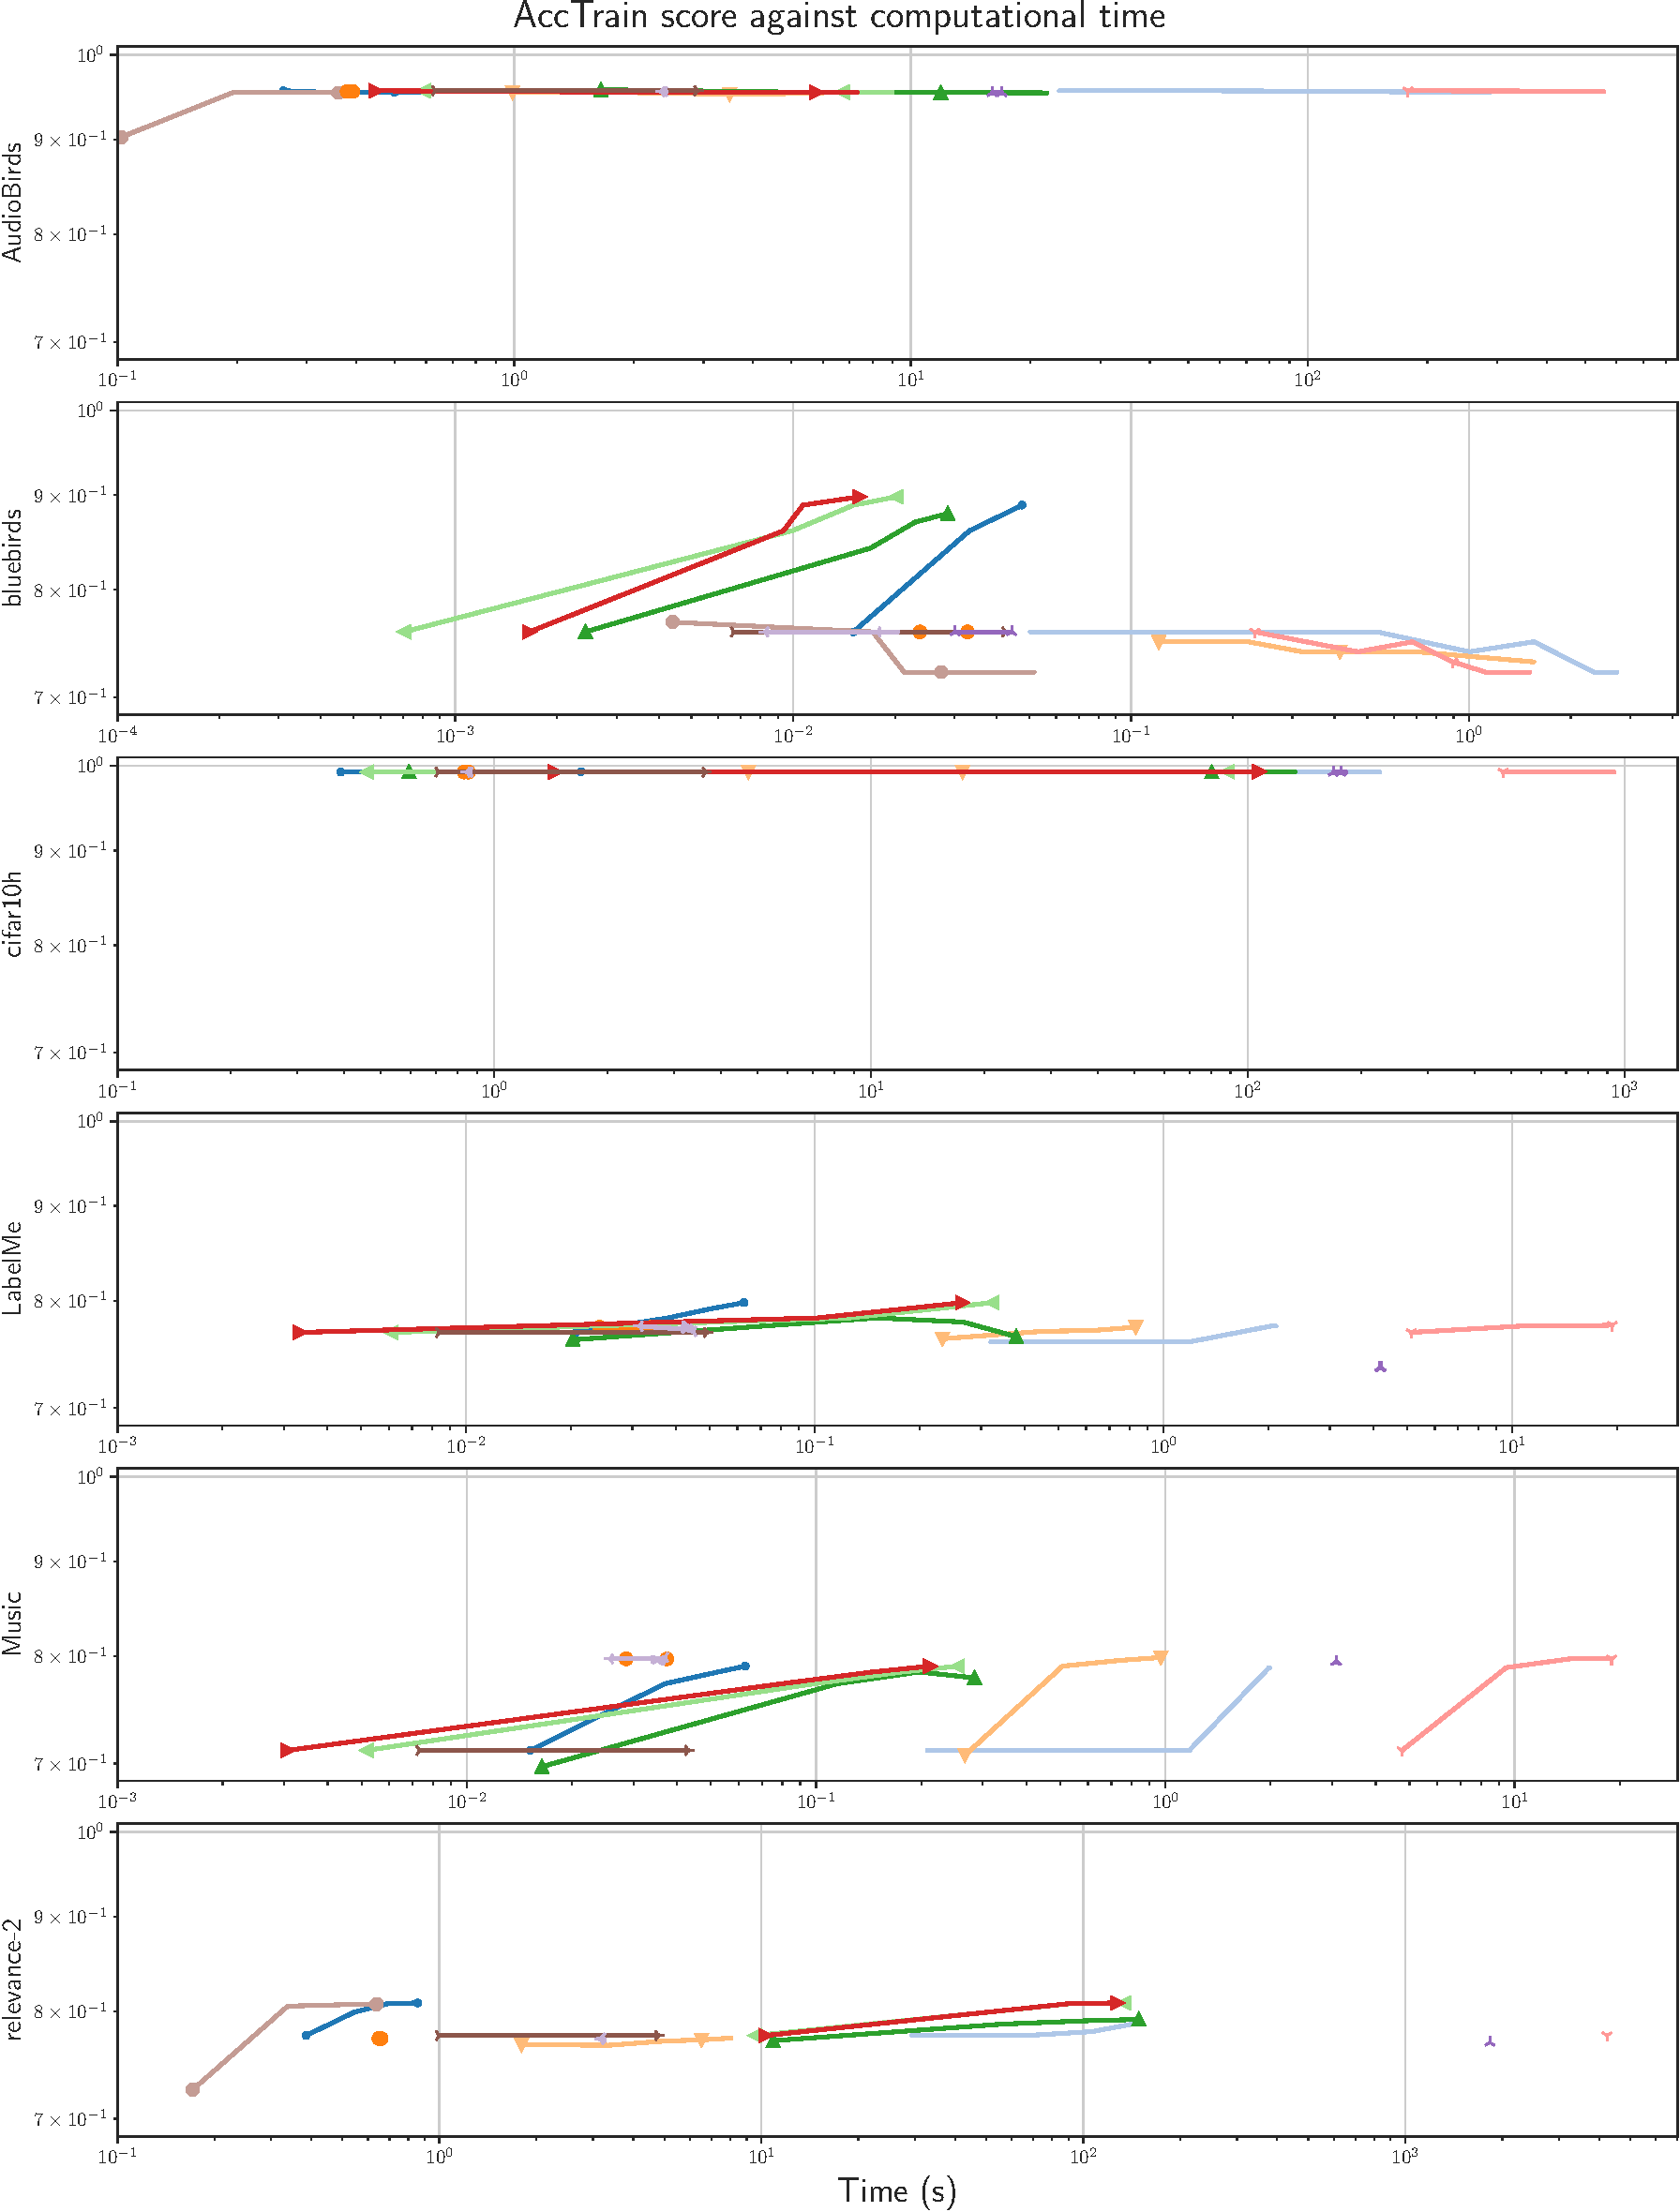
\includegraphics[width=\textwidth]{./chapters/images_benchopt/thesis_fig.pdf}
    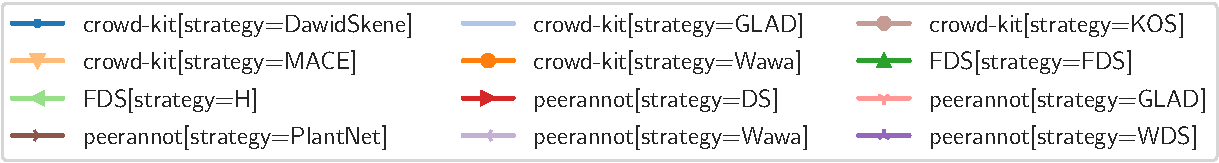
\includegraphics[width=\textwidth]{./chapters/images_benchopt/thesis_fig_legend.pdf}
    \caption{$\mathrm{AccTrain}$ score against computational time depending on the crowdsourced dataset and solver.}
    \label{fig:benchopt_crowd}
\end{figure}

Let us run the \texttt{Benchopt} library to compare the performance of different label aggregation strategies on multiple datasets.
We compare results from strategies within \texttt{peerannot}, \texttt{crowd-kit} and the Fast DS algorithms presented in \citet{sinha2018fast}.
A description of datasets, new solvers and more points of comparison between \texttt{peerannot} and \texttt{crowd-kit} is provided hereafter.

\subsubsection{Datasets and solvers information}

The list of all datasets compared in \Cref{fig:benchopt_crowd} is available in \Cref{tab:benchopt_datasets}.
We use Krippendorff's $\alpha\in[0,1]$ \citep{krippendorff1980validity} to measure the consistency in votes for each dataset.
A value over $0.8$ means a reliable dataset, between $0.6$ and $0.8$ the worker's answer includes inconsistencies.
A low value indicates high levels of disagreement and possibly unreliable data without the proper strategies according to \citet{krippendorff2004reliability}.

More formally, denoting $D_o$ the observed disagreement and $D_e$ the expected disagreement, Krippendorff's $\alpha$ is defined as:
\begin{equation}
    \alpha=1-\frac{D_o}{D_e} \enspace,
\end{equation}
with $D_o$ the observed disagreement and $D_e$ the expected disagreement.
In a classification setting, this formula writes:
\begin{equation}\label{eq:alphakripp}
    \alpha=\frac{(n-1)\displaystyle\sum_{c\in[K]}o_{c,c} - \displaystyle\sum_{c\in [K]} n_c(n_c-1)}{n(n-1) - \displaystyle\sum_{c\in [K]} n_c(n_c-1)} \enspace,
\end{equation}
with $n=\sum_{c\in [K]} n_c$, and $n_c=\sum_{k}o_{c,k}$ for $k\in [K]$ and
\[o_{c,k}= \sum_{i\in [n_\text{task}]}\frac{1}{|\mathcal{A}(x_i)|-1}|\{(c,k)\text{-pairs in task }i\}| \enspace.\]


\begin{table}[htbp]
    \centering
    \caption{Dataset information}
    \label{tab:benchopt_datasets}
    \begin{tabular}{lcccc}
        \toprule
        \textbf{Dataset} & $n_\text{worker}$ & $n_\text{task}$ &$K$ & Krippendorff's $\alpha$ \\
        \hline
        \hline
        AudioBirds \citep{lehikoinen2023successful} & 205 & 79 592 & 2 & 0.810 \\
        bluebirds \citep{WelinderEtal10b} & 39 & 108 & 2 & 0.126 \\
        relevance-2 & 7 138 & 99 319 & 2 & 0.262 \\
        CIFAR-10H \citep{peterson_human_2019} & 2 571 & 1000 & 10 & 0.910 \\
        LabelMe \citep{rodrigues2014gaussian} & 77 & 1000 & 8 & 0.677 \\
        Music \citep{rodrigues2017learning} & 44 & 700 & 10 & 0.301 \\
        \bottomrule
    \end{tabular}
\end{table}

In addition to presented solvers, we add in the comparison the Fast-DS solvers \citep{sinha2018fast}, KOS \citep{karger2011iterative}, the Multi-Annotator Competence Estimation (MACE) \citep{hovy2013learning} and Worker Agreement with Aggregate (WAWA) \footnote{\url{https://success.appen.com/hc/en-us/articles/202703205-Calculating-Worker-Agreement-with-Aggregate-Wawa}}.

\begin{constructionbox}[Computing Krippendorff's $\alpha$]
Let us consider a toy example with a dataset of $n_\text{task}=5$ tasks and $n_\text{worker}=3$ workers with $K=3$ classes. Some workers do not get to answer some of the tasks.
The votes are given as:

\begin{center}
\begin{tabular}{|c|ccccc|}
    \hline
    \textbf{Worker j / Task i} & \textbf{1} & \textbf{2} & \textbf{3} & \textbf{4} & \textbf{5} \\
    \hline
    1 &   & 1 & 1 & 2 & 1 \\
    2 & 0 & 1 &   &   & 0 \\
    3 & 0 & 2 &   & 2 & 0 \\
    4 & 0 &   & 1 & 2 & 2 \\
    \hline
    $|\mathcal{A}(x_i)|$ & 3 & 3 & 2 & 3 & 4 \\
    \hline
\end{tabular}
\end{center}

The class-coincidence matrix associated to this dataset is:

\begin{center}
\begin{minipage}[t]{0.45\textwidth}
\begin{center}
    \begin{tabular}{|c|ccc|c|}
        \hline
        \textbf{Classes} $c$ & 0 & 1 & 2 & $n_c$ \\
        \hline
        0 & $o_{0,0}$  & $o_{0,1}$ & $o_{0,2}$ & $n_0$ \\
        1 & $o_{1,0}$  & $o_{1,1}$ & $o_{1,2}$ & $n_1$\\
        2 & $o_{2,0}$  & $o_{2,1}$ & $o_{2,2}$ & $n_2$ \\
        \hline
    \end{tabular}
\end{center}
\end{minipage}
\hfill
$\Longleftrightarrow$
\hfill
\begin{minipage}[t]{0.45\textwidth}
\begin{center}
\begin{tabular}{|c|ccc|c|}
    \hline
    \textbf{Classes} $c$ & 0 & 1 & 2 & $n_c$ \\
    \hline
    0 & $\tfrac{11}{3}$ & $ \tfrac{2}{3}$ & $\tfrac{2}{3}$ & $5$ \\
    1 & $\tfrac{2}{3}$  & $3$ & $\tfrac{4}{3}$ & $5$\\
    2 & $\tfrac{2}{3}$  & $\tfrac{4}{3}$ & $3$ & $5$ \\
    \hline
\end{tabular}
\end{center}
\end{minipage}
\end{center}

Let us detail two examples:
\begin{itemize}
    \item $o_{0,0}$: In the first task there are $6$ pairs of $(0,0)$ agreements over $3$ answers. In the tasks $2,3,4$ there are no votes for class $0$. And for task $5$ there are $2$ pairs of $(0,0)$ agreements over $4$ answers. Hence $o_{0,0}=\frac{6}{3-1} + \frac{2}{4-1}=\frac{6}{2} + \frac{2}{3}=\frac{11}{3}$.
    \item $o_{2,1}$: In the tasks $1$, $3$ and $4$ there are no $(2,1)$ disagreements. In task $2$ there are $2$ pairs of $(2,1)$ disagreements over $3$ answers. And in task $5$ there is $1$ pair of $(2,1)$ disagreements over $4$ answers. Hence $o_{2,1}=\frac{2}{3-1} + \frac{1}{4-1}=\frac{2}{2} + \frac{1}{3}=\frac{4}{3}$.
\end{itemize}
Finally, we use \Cref{eq:alphakripp} and obtain with $n=5+5+5=15$:
\begin{align*}
\alpha  &= \frac{(n-1)\left(\frac{11}{3} + 3 + 3\right) - \left(5(5-1)  + 5(5-1) + 5(5-1)\right)}{n(n-1) - \left(5(5-1)  + 5(5-1) + 5(5-1)\right)} \\
        &\simeq 0.502 \enspace.
\end{align*}
Hence this data is quite unreliable.

Note that in settings other than classical classification (\emph{e.g.} ranking) the coincidence matrix might not be symmetrical.
See \citet{krippendorff1980validity} for forms of $\alpha$ expression instead of \Cref{eq:alphakripp}.
\end{constructionbox}

Let us present the additional label aggregation strategies briefly. The PlantNet aggregation is presented in detail in \Cref{chap:plantnet}.
\paragraph{WAWA.}
This strategy, also known as the inter-rater agreement, weights each user by how much they agree with the MV labels on average. More formally, given a task $i$:
\begin{align*}
    \mathrm{WAWA}(i, \mathcal{D}) &= \argmax_{k\in [K]} \sum_{j\in \mathcal{A}(x_i)} \beta_j\mathds{1}(y_i^{(j)} = k) \\
    \text{with } \beta_j &= \frac{1}{|\{y_{i'}^{(j)}\}_{i'}|} \sum_{i'=1}^{n_{\mathrm{task}}} \mathds{1}\left(y_{i'}^{(j)} = \mathrm{MV}(i', \{y_{i'}^{(j)}\}_j)\right)\enspace.
    \end{align*}

Note that even if they are not iterative strategies WAWA and WDS can still be shown in \texttt{Benchopt}.
However, the performance is computed at the end of the aggregation process, and only the first point of the curve should be considered. Indeed, the second point is an artifact from \texttt{Benchopt}'s stopping criterion (the patience) described in \Cref{sub:benchopt_how}.

\paragraph{MACE \citep{hovy2013learning}.}

\begin{figure}[tbh]
    \centering
    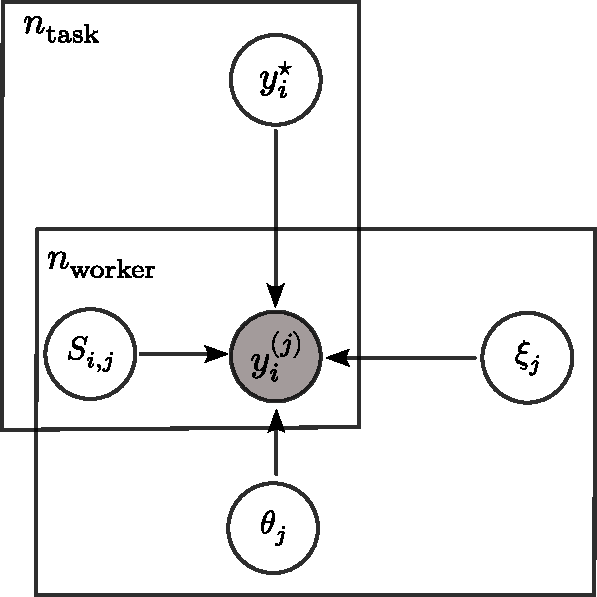
\includegraphics[height=8cm, keepaspectratio]{./images_benchopt/mace_plate.pdf}
    \caption{Bayesian plate diagram representation of the MACE model. Only the labels $\{y_i^{(j)}\}_{i,j}$ are observed. Latent variables to estimate are the true labels ($y_i^\star$), the spamming state $(S_{i,j})_{i,j}$, the probability to spam $(\theta_j)_j$ and the worker behavior when spamming $(\xi_j)_j$.}
    \label{fig:plate_mace}
\end{figure}

The MACE strategy has been designed to be more robust against spammers.
Contrary to the definition of spammers by \citet{raykar_ranking_2011}, they here consider spam as a state of the worker.

Each worker can be spamming on each task. The probability for a worker to spam a task is given by a Bernoulli distribution with parameter $1-\theta_j\in[0, 1]$. Thus, denoting $S_{i,j}$ the spamming state of worker $j$ on task $i$, the probability of the worker to spam the task is drawn as $S_{i,j}\sim\mathcal{B}(1-\theta_j)$. If a worker is not spamming ($S_{i,j}=0$) then they answer the correct underlying label $y_i^\star$. If not, their answer is drawn at random from a multinomial distribution with parameter $\xi_j\in\Delta_{K}$ proper to each worker.
For a given worker $j_0$, the distribution $\xi_{j_0}$ indicates what is their behavior when they are spamming.

The associated likelihood -- maximized using the EM algorithm as in DS -- writes:
\begin{align*}
\mathbb{P}(\{y_i^{(j)}\}_{i,j}|\theta,\xi) =& \\ \sum_{y^\star\in [K]^{n_\text{task}}}&\sum_{S\in\{0,1\}^{n_\text{task}\times n_\text{worker}}}\left[\prod_{i=1}^{n_\text{task}} \mathbb{P}(y^\star_i) \prod_{j=1}^{n_\text{worker}} \mathbb{P}(S_{i,j}|\theta_j)\mathbb{P}(y_i^{(j)}|S_{i,j},y_i^\star, \xi_j)\right]\enspace.
\end{align*}

In \Cref{fig:plate_mace}, we represent the associated bayesian plate diagram.

\paragraph{KOS \citep{karger2011iterative}.}
Only set for binary classification $y_i^\star\in\{\pm 1\}$, the KOS strategy is from a graph-theory perspective.
Denote $G([n_\text{task}]\cup [n_\text{worker}], E)$ the graph where edge $(i,j)$ is connected if worker $j$ has answered task $i$. The neighborhood of a task $i$ is denoted $\partial_i$ and the same with index $j$ for workers.
On each edge is stored the label answered by worker $j$ for task $i$: $y_i^{(j)}\in[K]$.

The KOS strategy estimates how much a worker is reliable by how much their answers are consistent with the answers of their neighbors and the likelihood of a task having $y_i^\star=1$.
Both pieces of information are propagated into the graph as messages.
The final label is then estimated by the sign of the sum of the messages received by the task weighted by the workers' reliability.

A task message denoted $x_{i\rightarrow j}$ is the log-likelihood of the task $i$ having $y_i^\star=1$.
A worker message denoted $y_{j\rightarrow i}$ is the reliability of worker $j$.
Both messages have scalar values.
After random initialization, the messages are updated iteratively until convergence following the equations:
\begin{align*}
    x_{i\rightarrow j} &\gets \sum_{j'\in \partial_i\setminus \{j\}} y_i^{(j')}y_{j'\rightarrow i} \ \forall (i,j)\in E \\
    y_{j\rightarrow i} &\gets \sum_{i'\in \partial_j\setminus \{i\}} y_{i'}^{(j)} x_{i'\rightarrow j} \ \forall (i,j)\in E\enspace.
\end{align*}
Finally, the estimated label is computed as:
\[
\forall i\in [n_\text{task}],\ \hat y_i^{\text{KOS}} = \mathrm{sign}\left(\sum_{j\in\partial_i} y_i^{(j)}y_{j\rightarrow i}\right)\enspace.
\]

\begin{constructionbox}[Visualizing KOS.]
Let us consider the binary answers:
\begin{center}
\begin{tabular}{|c|ccccc|}
    \hline
    \textbf{Worker j / Task i} & \textbf{1} & \textbf{2} & \textbf{3} & \textbf{4} & \textbf{5} \\
    \hline
    1 &    & 1  & 1  & -1  &  1 \\
    2 & -1 & 1  &    &     &  1 \\
    3 & 1  & 1  &    & 1   &  1 \\
    4 & -1 &    & 1  & -1  & -1 \\
    \hline
\end{tabular}
\end{center}

The associated graph representing workers in blue and tasks in red is:

\begin{minipage}[c]{0.40\textwidth}
    \begin{center}
    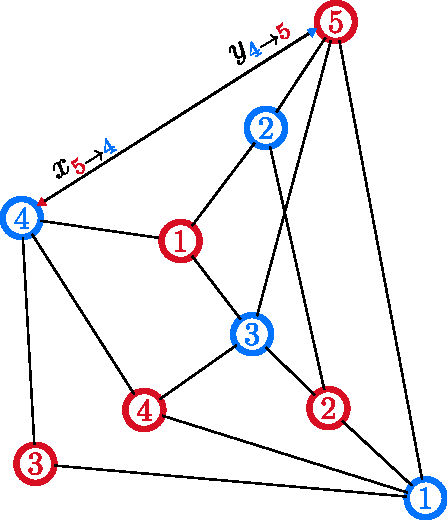
\includegraphics[width=\textwidth]{./images_benchopt/network_kos.pdf}
    \end{center}
    \end{minipage}\hfill
    \begin{minipage}[c]{0.45\textwidth}
    Each task sends a message $x_{i\rightarrow j}$ to each worker who answered them. Each worker sends a message $y_{j\rightarrow i}$ to each task they answered.

    For example, task $5$ sends messages to workers $4,3,2$ and $1$

    Thus $\partial_{\textcolor{red}{5}}=\{1,2,3,4\}$.

    Worker $4$ sends messages to tasks $1,3,4$ and $5$.

    Thus $\partial_{\textcolor{blue}{4}}=\{1,3,4,5\}$.
\end{minipage}

\smallskip

At a given step, the reliability of worker $\textcolor{blue}{4}$ concerning their answer to task $\textcolor{red}{5}$ is thus updated as follows:
\[
    y_{\textcolor{blue}{4}\rightarrow \textcolor{red}{5}} = \sum_{i'\in \partial_{\textcolor{blue}{4}}\setminus \{\textcolor{red}{5}\}} y_{i'}^{(\textcolor{blue}{4})} x_{i'\rightarrow \textcolor{blue}{4}} = -1\times x_{\textcolor{red}{1}\rightarrow \textcolor{blue}{4}} + 1\times x_{\textcolor{red}{3}\rightarrow \textcolor{blue}{4}} + (-1)\times x_{\textcolor{red}{4}\rightarrow \textcolor{blue}{4}}  + (-1)\times x_{\textcolor{red}{5}\rightarrow \textcolor{blue}{4}}\enspace.
\]
\end{constructionbox}

\paragraph{Fast-DS \citep{sinha2018fast}.}
As the DS strategy is known to have a high computational cost, \citet{sinha2018fast} proposed a faster version of the DS strategy.
The Fast-DS strategy is based on the same principle as DS, but the computation of the posterior distribution on the estimated ground truth is restricted as a Dirac distribution.
Note that this does not alleviate the memory issue of the DS strategy -- the $K^2\times n_{\text{worker}}$ parameters to estimate for the confusion matrices.
Under the assumption that there is only a single label per task -- which is the case in this thesis -- this \emph{hard} version of the DS strategy claims to be faster than the original DS strategy while achieving similar performance in accuracy.

More formally, following the DS notation from \Cref{subsub:ds} the Fast-DS method adds the following step in the ground truth estimation:
\[
T_{i,k} = \begin{cases} 1 & \text{if } k = \displaystyle\argmax_{k'\in[K]} \mathbb{P}\left(y_i^\star=k'|\{y_i^{(j)}\}_{j\in\mathcal{A}(x_i)}\right) \\ 0 & \text{otherwise} \end{cases} \enspace.
\]
The quantity $\mathbb{P}\left(y_i^\star=k'|\{y_i^{(j)}\}_{j\in\mathcal{A}(x_i)}\right)$ is estimated using Baye's theorem.

However, empirical results show that the Fast-DS strategy with this \emph{hard} decision can reach lower accuracy.
To alleviate this convergence issue, \citet{sinha2018fast} proposed to use a \emph{hybrid} version of the Fast-DS strategy.
The hybrid strategy is defined as:
\begin{itemize}
    \item Run the classical DS algorithm first to estimate the marginal class likelihood $\rho\in\Delta_K$ at each iterate.
    \item When the absolute difference between two consecutive iterates of $\rho$ is lower than a given threshold, switch to the \emph{hard} version of the DS strategy.
\end{itemize}
This hybrid strategy allows having a softer control on the label estimation at the beginning and better exploring the latent variable's space.
Finishing with \emph{hard} labels allows faster convergence.
However, in practice this gain -- as seen in \Cref{fig:benchopt_crowd} -- can be mitigated by the implementation of the DS strategy.

\paragraph{Results interpretation.}
Running \texttt{Benchopt} evaluation, we obtain \Cref{fig:benchopt_crowd} showing the accuracy of the different label aggregation strategies against the computational time.
Depending on the dataset, some solvers -- \emph{i.e.} label aggregation strategy -- are more suited and less computationally expansive than others.

For example, on the \texttt{BlueBirds} dataset, \texttt{peerannot}'s DS strategy is the fastest to reach the best accuracy. It is followed by the Fast-DS and then \texttt{crowd-kit}'s DS aggregation.
As the $\alpha$ value is very low ($\alpha=0.126$), the dataset is unreliable.
Hence, strategies that are specific to some workers' behaviors -- KOS for spammers, GLAD for ambiguous tasks -- are not suited and the DS strategy seems to be the best choice.

In the case of datasets with a high level of agreement ($\alpha>0.8$) -- in AudioBirds and CIFAR-10H -- all strategies reach the level of performance. Notice that GLAD is again slower than most strategies (this conclusion can be seen in most cases). For those datasets, the simpler the strategy, the faster the same level of accuracy.

For the \texttt{Music} dataset, the best performance is achieved by the fastest method in this case: $\mathrm{WAWA}$ (with similar time computation between \texttt{peerannot} and \texttt{crowd-kit}).
And finally, for the \texttt{LabelMe} dataset, the best performance is achieved by the DS-based strategies.
WAWA aggregation underperforms: as shown in \Cref{fig:LabelMe_dataset_visualization}, the tasks have very few labels and are ambiguous with the class overlap.

Overall, the Pl@ntNet strategy does not perform better than other label aggregation strategies. This is because the algorithm is not suited for such crowdsourced datasets. It is based on the assumption that the number of possible classes is high to evaluate the worker's reliability. This is not the case in the datasets we consider. We have at most $K=10$. Hence why in \Cref{chap:plantnet} we released a large subset of Pl@ntNet's database to evaluate this strategy on a more suitable dataset.

\subsubsection{More comparison between \texttt{peerannot} and \texttt{crowd-kit}.}

Both \texttt{peerannot} and \texttt{crowd-kit} are open-source libraries to handle crowdsourced datasets.
While \texttt{crowd-kit} proposes segmentation and regression crowdsourcing strategies, \texttt{peerannot} is focused on classification tasks.
The learning strategies (CrowdLayer and CoNAL) are available in both libraries, and each library has label aggregations strategies with some in common (MV, GLAD, DS, WAWA) and some library-specific (Pl@ntNet, WDS, KOS, MACE).
However, the main difference between the two libraries is the identification step. So let us focus on this.

At the time of writing \texttt{crowd-kit} proposes four strategies to explore crowdsourced datasets:
\begin{itemize}
    \item Krippendorff's $\alpha$: to measure the consistency in votes for each dataset (also available in \texttt{peerannot}).
    \item The consistency: Averaged posterior distribution of a label determination from workers' estimated reliability.
    \item The uncertainty: the entropy of the distribution of the votes (also available in \texttt{peerannot}).
    \item The accuracy of aggregates: the accuracy of a subset of worker's answers from aggregated labels (if the subset of workers is all workers and the aggregated label is the MV label, this simplifies as the weight of users in WAWA).
\end{itemize}

In \texttt{peerannot}, we added:
\begin{itemize}
    \item The $\mathrm{AUMC}$: deep learning based ambiguity score on tasks via MV aggregation (see \Cref{chap:waum}).
    \item The $\mathrm{WAUM}$: deep learning based ambiguity score on tasks via weighted Areas Under the Margin (see \Cref{chap:waum}).
    \item The spam score \citep{raykar_ranking_2011}: distance between the estimated confusion matrix and the closest rank-$1$ matrix for each worker. This allows identifying potential spammers.
    \item The trace confusion: sum of the diagonal terms of the DS confusion matrices. Indicates the level of reliability per worker for their answered label. The closer the trace to $K$, the more reliable the worker.
\end{itemize}

The \texttt{peerannot} library also supports top-$k$ classification metrics for deep-learning methods.
We provide the \texttt{train} command to train deep learning models from \texttt{TorchVision} on the dataset and evaluate their accuracy and calibration if a test set is available. This allows users to have a fully end-to-end pipeline:
\begin{itemize}
    \item identify potential ambiguous tasks / bad workers,
    \item aggregate the labels and train a computer vision network,
    \item or directly train a computer vision network with deep-learning-based strategies to handle crowdsourced tasks.
\end{itemize}
Keeping the same framework from beginning to end, based on PyTorch, allows for a more seamless integration of the crowdsourcing pipeline in existing projects.

As we will see in \Cref{chap:plantnet}, the \texttt{peerannot} library is more suited for classification tasks with a high number of classes, tasks and/or workers. Indeed, for the dataset we will consider, none of the aggregation strategies from \texttt{crowd-kit} could be run due to memory issues that are directly linked to the data format choice.

\section{Conclusion}

We presented the \texttt{peerannot} library: an open-source \texttt{python} library to handle crowdsourced datasets.
This library is designed to be modular and to allow easy integration of new label aggregation strategies, learning strategies and identification strategies on new datasets.

To produce fair and reproducible comparisons of label aggregation strategies' performance, we added a new benchmark to the \texttt{Benchopt} library.
This benchmark for crowdsourcing in classification problems allows us to compare the performance of different label aggregations depending on the ambiguity of a dataset.
We showed that the \texttt{peerannot} library is a good candidate to handle crowdsourced datasets against standalone openly available methods (FDS) or other libraries like \texttt{crowd-kit}.

